% Options for packages loaded elsewhere
\PassOptionsToPackage{unicode}{hyperref}
\PassOptionsToPackage{hyphens}{url}
\documentclass[
]{article}
\usepackage{xcolor}
\usepackage{amsmath,amssymb}
\setcounter{secnumdepth}{-\maxdimen} % remove section numbering
\usepackage{iftex}
\ifPDFTeX
  \usepackage[T1]{fontenc}
  \usepackage[utf8]{inputenc}
  \usepackage{textcomp} % provide euro and other symbols
\else % if luatex or xetex
  \usepackage{unicode-math} % this also loads fontspec
  \defaultfontfeatures{Scale=MatchLowercase}
  \defaultfontfeatures[\rmfamily]{Ligatures=TeX,Scale=1}
\fi
\usepackage{lmodern}
\ifPDFTeX\else
  % xetex/luatex font selection
\fi
% Use upquote if available, for straight quotes in verbatim environments
\IfFileExists{upquote.sty}{\usepackage{upquote}}{}
\IfFileExists{microtype.sty}{% use microtype if available
  \usepackage[]{microtype}
  \UseMicrotypeSet[protrusion]{basicmath} % disable protrusion for tt fonts
}{}
\makeatletter
\@ifundefined{KOMAClassName}{% if non-KOMA class
  \IfFileExists{parskip.sty}{%
    \usepackage{parskip}
  }{% else
    \setlength{\parindent}{0pt}
    \setlength{\parskip}{6pt plus 2pt minus 1pt}}
}{% if KOMA class
  \KOMAoptions{parskip=half}}
\makeatother
\usepackage{graphicx}
\makeatletter
\newsavebox\pandoc@box
\newcommand*\pandocbounded[1]{% scales image to fit in text height/width
  \sbox\pandoc@box{#1}%
  \Gscale@div\@tempa{\textheight}{\dimexpr\ht\pandoc@box+\dp\pandoc@box\relax}%
  \Gscale@div\@tempb{\linewidth}{\wd\pandoc@box}%
  \ifdim\@tempb\p@<\@tempa\p@\let\@tempa\@tempb\fi% select the smaller of both
  \ifdim\@tempa\p@<\p@\scalebox{\@tempa}{\usebox\pandoc@box}%
  \else\usebox{\pandoc@box}%
  \fi%
}
% Set default figure placement to htbp
\def\fps@figure{htbp}
\makeatother
\setlength{\emergencystretch}{3em} % prevent overfull lines
\providecommand{\tightlist}{%
  \setlength{\itemsep}{0pt}\setlength{\parskip}{0pt}}
\usepackage{bookmark}
\IfFileExists{xurl.sty}{\usepackage{xurl}}{} % add URL line breaks if available
\urlstyle{same}
\hypersetup{
  hidelinks,
  pdfcreator={LaTeX via pandoc}}

\author{}
\date{}

\begin{document}

{Introduzione}

{L'obiettivo del PT è trovare e utilizzare vulnerabilità all'interno
dell'applicativo web }{OWASP Juice Shop}{.}

{Oltre a questo report verranno allegati }{i file di output dei vari
tool utilizzati}{.}

{}

{Metodologia}

{Di seguito descriviamo step-by-step le fasi del penetration test}

\section{\texorpdfstring{{Information
Gathering}}{Information Gathering}}\label{h.nvejnwrrrvn3}

{Tecniche e strumenti utilizzati per raccogliere informazioni iniziali.}

{}

{}

{Abbiamo iniziato utilizzando }{Nmap }{per fare }{Service Enumeration}{,
specificando l'ip della web app e la porta con il comando:}

{}

{sudo nmap -p3000 -sV -O 172.17.0.2}

{}

{senza però ottenere risultati utili (file: }{nmapOutput.txt}{).}

{}

{}

{Per cercare di trovare qualche tecnologia utilizzata (con relative
versioni) abbiamo utilizzato Wappalyzer, ottenendo:}

{\pandocbounded{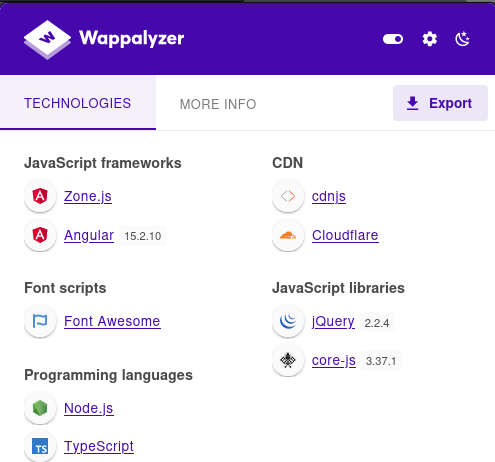
\includegraphics[keepaspectratio]{images/image3.png}}}

{Dal tool otteniamo solo 3 versioni, e cercando nel web vulnerabilità
specifiche troviamo:}

\begin{itemize}
\tightlist
\item
  {Angular 15.2.10}{: nessuna vulnerabilità;}
\item
  {jQuery 2.2.4}{: vulnerabile ad attacchi di tipo }{Cross-site
  Scripting (XSS)}{;}
\item
  {core-js 3.37.1}{: nessuna vulnerabilità.}
\end{itemize}

{In sostanza terremo utile questa unica informazione per le fasi
successive.}

{}

{Un altro tool utilizzabile per scovare informazioni sulla web app è
}{WhatWeb}{:}

{\pandocbounded{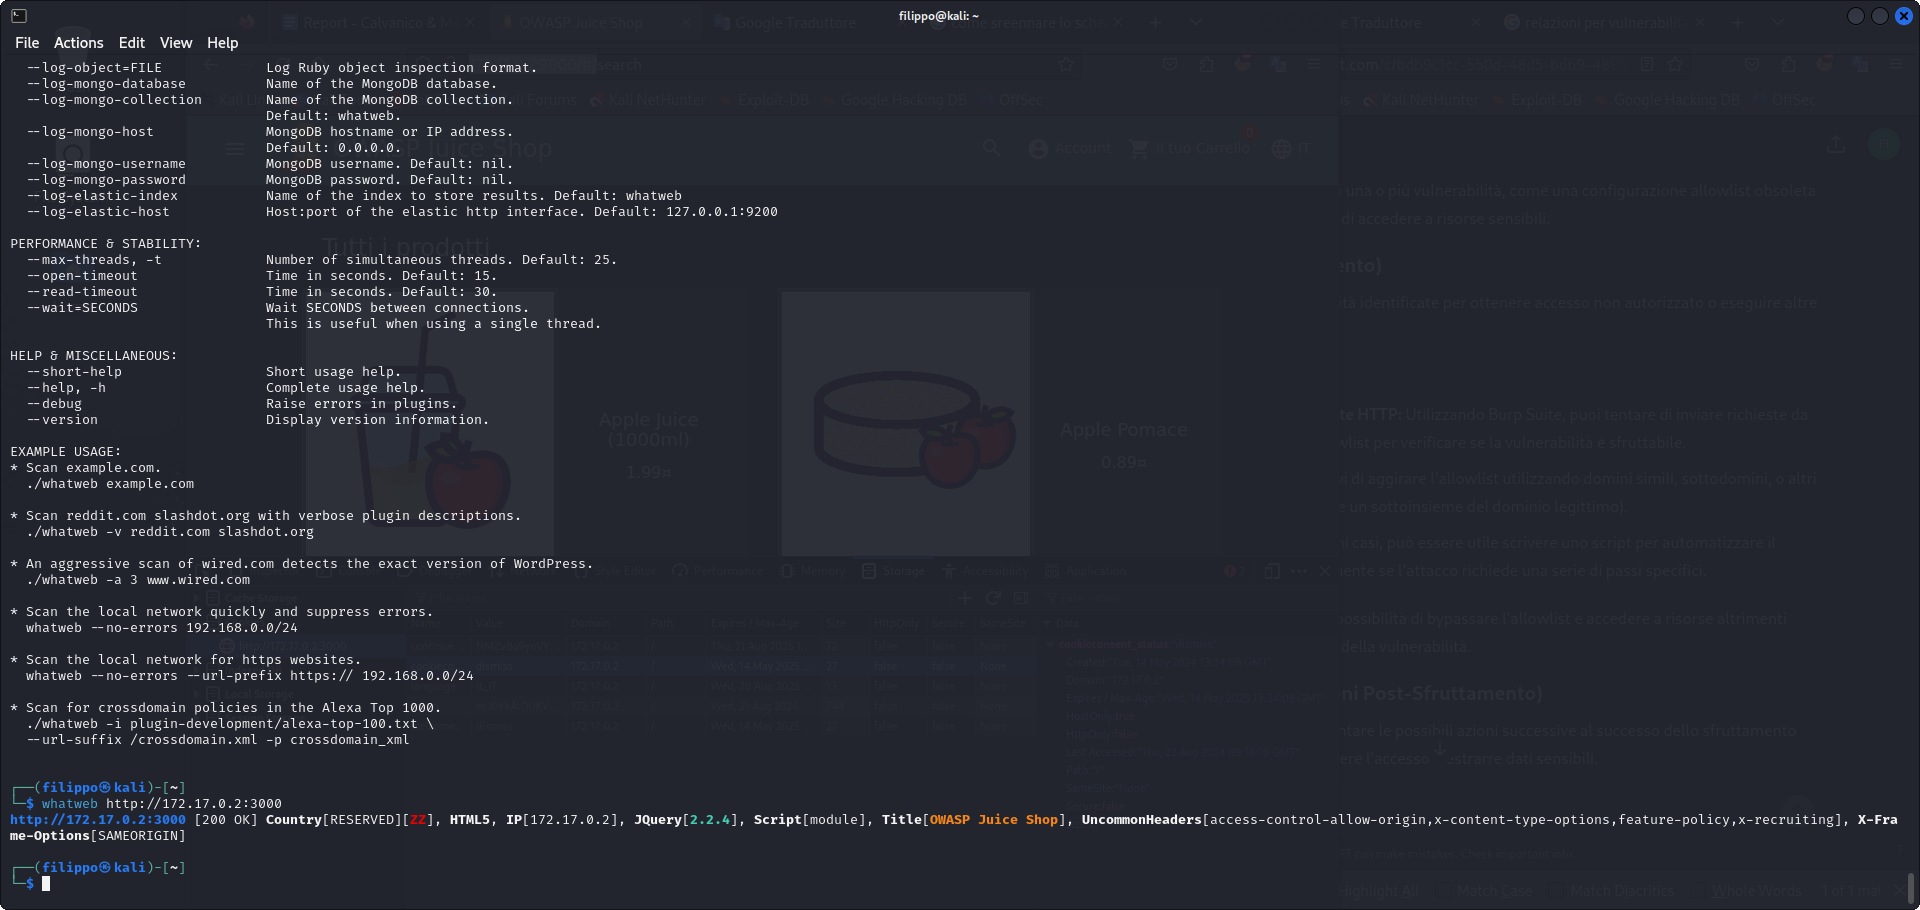
\includegraphics[keepaspectratio]{images/image1.png}}}

{}

{}

{Il passo successivo è }{controllare,}{~tramite }{WAFW00F}{, se
l'applicazione ha un WAF (Web Application Firewall), e tramite il
comando:}

{}

{wafw00f
}{\href{https://www.google.com/url?q=http://172.17.0.2:3000&sa=D&source=editors&ust=1734622045274776&usg=AOvVaw3CDavK8M_iUKxEgvH4rrIz}{http://172.17.0.2:3000}}

{}

{abbiamo ottenuto una risposta negativa che quindi ci conferma che non è
presente un WAF (file: }{outputWafw00f.txt}{).}

{}

{Per avere un ulteriore conferma che le risposte http non vengano
alterate e capire se c'è uno strumento di detection/response tramite
l\textquotesingle utilizzo di Wireshark abbiamo filtrato le risposte
HTTP, notando che la prima richiesta fatta è classica, per poi andare ad
eseguire altre richieste con dei failed, ad esempio }{``Ealert''.}

{\pandocbounded{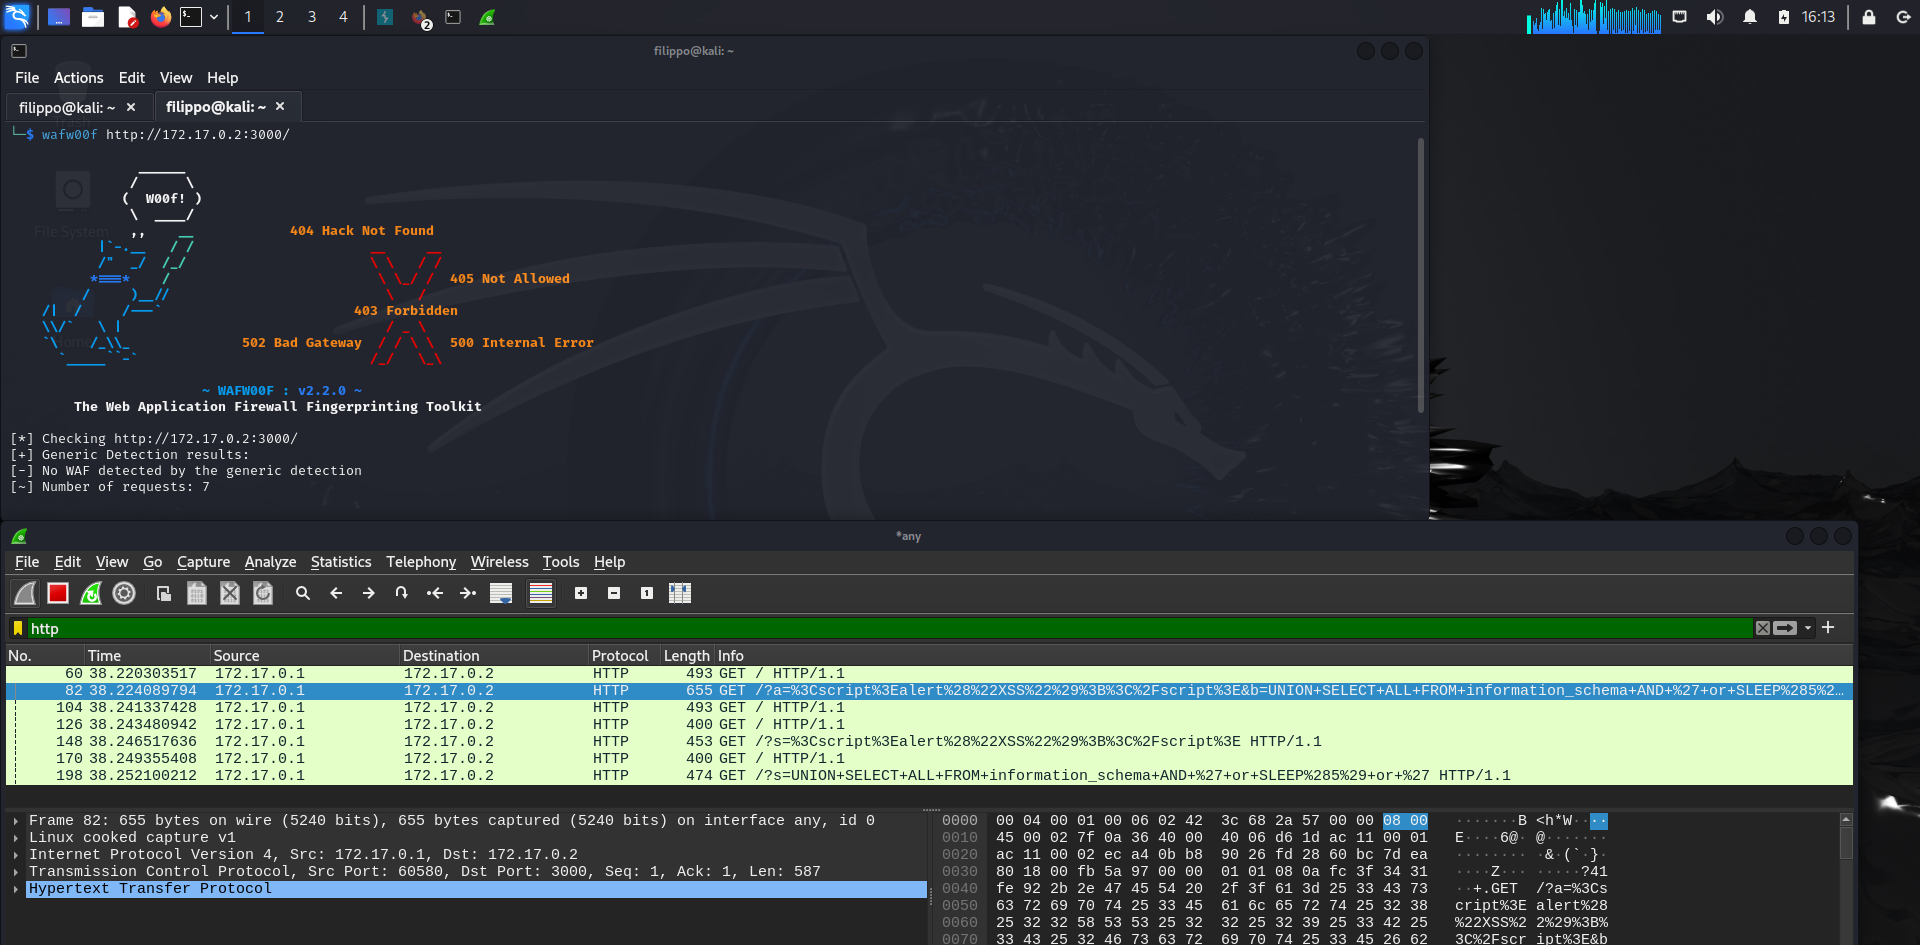
\includegraphics[keepaspectratio]{images/image15.png}}}

{}

{}

{Per cercare alcuni path o file interessanti abbiamo usato }{Nikto}{,
ottenendo un gran numero di falsi positivi ma anche risultati (file:
}{outputNikto}{),}{~in particolare:}

\begin{itemize}
\tightlist
\item
  {/ftp}{: contiene molti file non leggibili, ma tra quelli leggibili
  abbiamo ``}{acquisitions.md}{'' un file confidenziale. L'apertura dei
  file non leggibili ci permette di scoprire, tramite errore, che la web
  app usa }{Express 4.17.1}{;}
\end{itemize}

{\pandocbounded{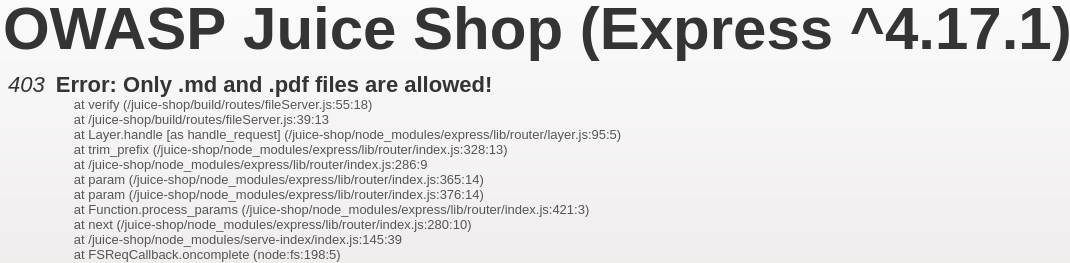
\includegraphics[keepaspectratio]{images/image31.png}}}

{Vulnerabile ad attacchi di tipo }{Open Redirect}

{}

\begin{itemize}
\tightlist
\item
  {/ftp/quarantine}{: directory con malware per diversi OS;}
\end{itemize}

{\pandocbounded{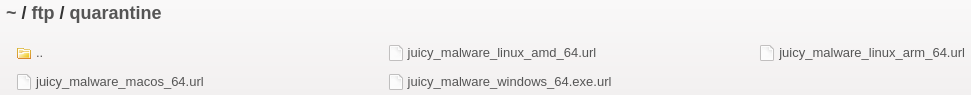
\includegraphics[keepaspectratio]{images/image17.png}}}

{Successivamente siamo passati alla pagina di login cercando, in qualche
modo, di provocare errori che ci avrebbero dato indizi sulle tecnologie
o metodologie utilizzate nel backend. }

{Inserendo caratteri inaspettati dalla }{form,}{~come per esempio il
singolo apice, abbiamo ottenuto un errore diverso dal solito, che ci fa
capire come probabilmente c'è un problema che potrebbe portarci ad una
vulnerabilità.}{\pandocbounded{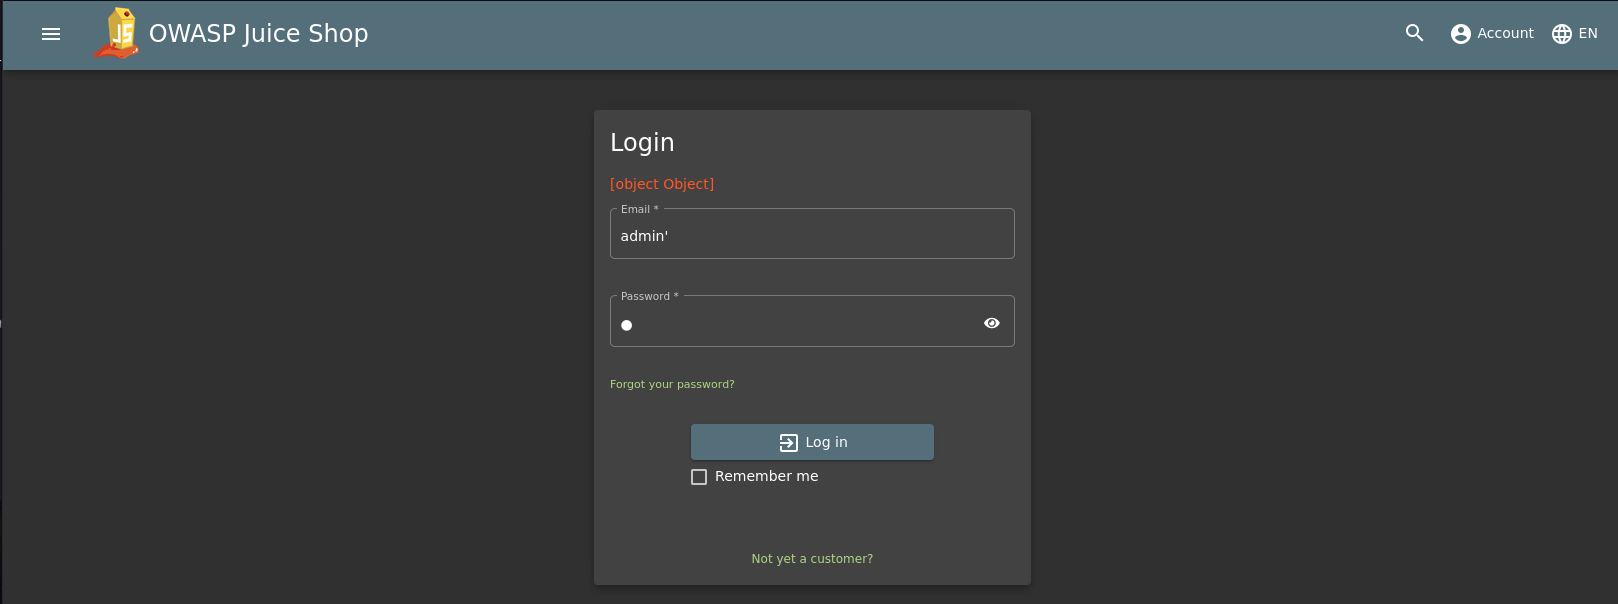
\includegraphics[keepaspectratio]{images/image21.png}}}

{Nella parte di vulnerability assessment indagheremo meglio.}

{}

{}

{Il passo successivo è stato quello di trovare nuove directory e
sottodirectory tramite tool automatizzati, nel nostro caso }{Ffuf}{~
(file: }{outputFfuf}{),}{~dove tramite comando:}

{}

{ffuf -u }{http://172.17.0.2:3000/FUZZ}{~-w
/usr/share/dirbuster/wordlists/directory-list-1.0.txt ~-fs 3740-3750}

{}

{abbiamo cercato all'interno della web app tutti i possibili percorsi,
passandogli una wordlist (contenuta nativamente dentro kali) con parole
chiave da cercare e togliendo tutti i risultati che ritornavano una size
compresa tra quella inserita (la size della homepage); questo perché il
sito ritorna la pagina iniziale ogni volta che si prova ad accedere ad
un indirizzo inesistente.}

{Tra i path trovati quelli effettivamente raggiungibili e interessanti
sono:}

\begin{itemize}
\tightlist
\item
  {/restoration}{: path che ritorna un errore e come i precedenti ci da
  informazioni sul backend;}
\end{itemize}

{}

\begin{itemize}
\tightlist
\item
  {/apictureofbritain}{:}{~come il precedente}
\end{itemize}

{}

\begin{itemize}
\tightlist
\item
  {/video}{: ci mostra un video altrimenti non raggiungibile;}
\end{itemize}

{}

\begin{itemize}
\tightlist
\item
  {/metrics}{: un'insieme di metriche di nodejs}{;}
\end{itemize}

{}

\begin{itemize}
\tightlist
\item
  {/redirect}{: da questo path se aggiunto }{?to=}{~è possibile arrivare
  a parti altrimenti non raggiungibili, questo perchè i bottoni
  utilizzano questa combinazione per portare in altre pagine, tramite
  Burp lo possiamo
  dimostrare}{.}{\pandocbounded{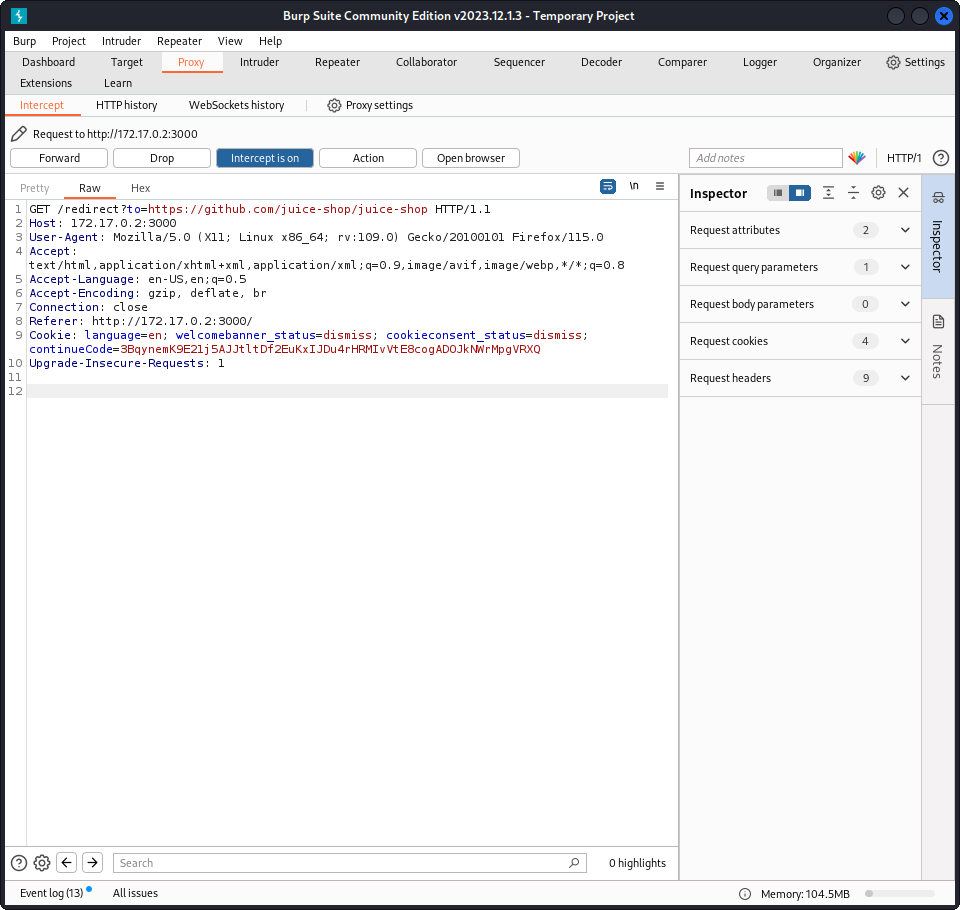
\includegraphics[keepaspectratio]{images/image22.png}}}
\end{itemize}

{}

{}

{Notando che alcune pagine contenevano nel path: }{/\#/nome}{~abbiamo
pensato di fare nuove scansioni (file: }{outputFfuf2.txt)}{,}{~sempre
con fuff però usando un link diverso e con delle wordlist differenti
(relative al tool):}

{}

{ffuf -u }{http://172.17.0.2:3000/\#/FUZZ}{~-w
/usr/share/wfuzz/wordlists/common.txt ~-}{o outputFfuf2.txt}

{}

{In questo caso abbiamo tolto il filtro perché con esso non dava
risultati.}

{Togliendo il filtro otteniamo molti falsi positivi, ma dopo aver
controllato alcuni }{path}{~interessanti abbiamo trovato:}

\begin{itemize}
\tightlist
\item
  {/administration}{: il path ritorna errore 403, questo vuol dire che
  esiste ma non è accessibile senza permessi, sarà da ricontrollare dopo
  aver fatto l'accesso}{;}
\end{itemize}

{}

{}

{Infine controlliamo anche i cookie per cercare nei flag eventuali
parametri non conformi da utilizzare per scovare vulnerabilità, senza
però riscontrare nulla di anomalo.}

{\pandocbounded{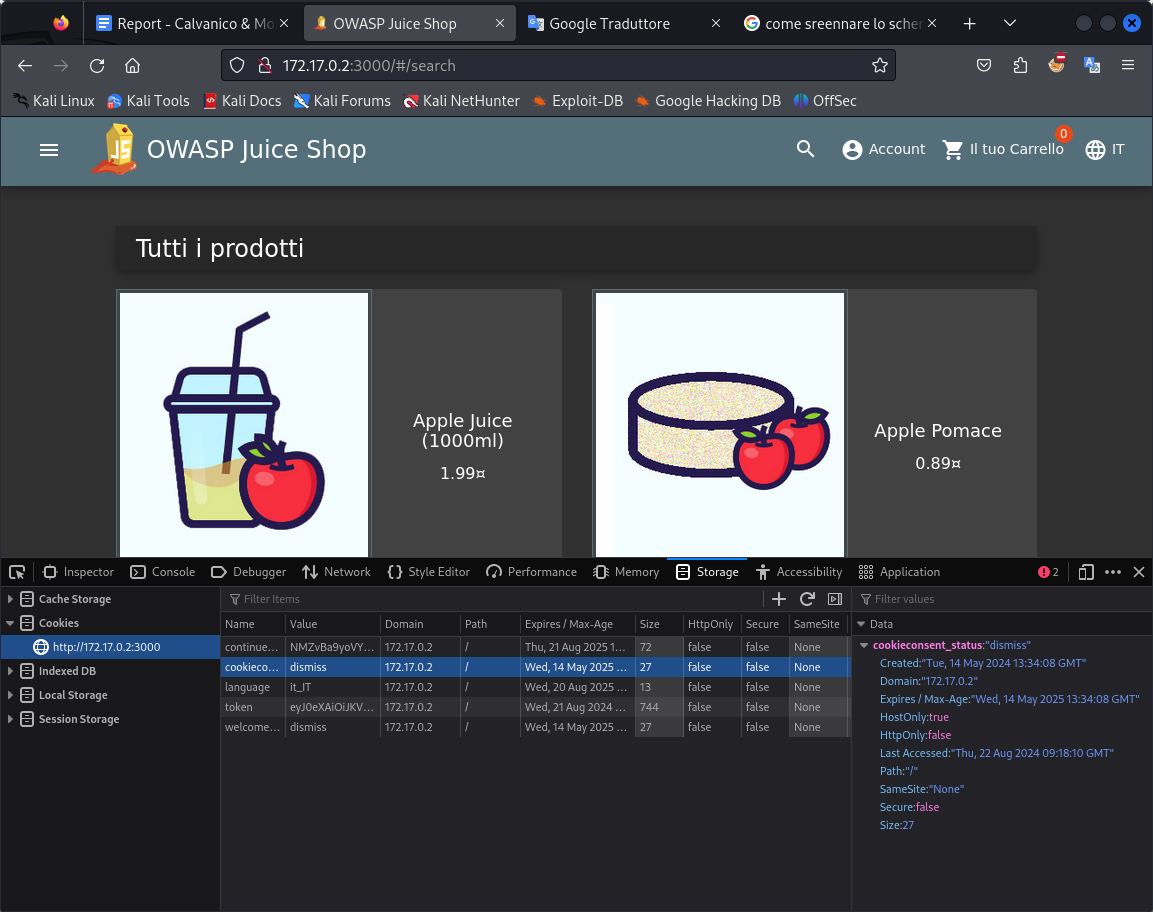
\includegraphics[keepaspectratio]{images/image25.png}}}

\section{\texorpdfstring{{Vulnerability
Assessment}}{Vulnerability Assessment}}\label{h.uqvtt1sn73zs}

{Strumenti e metodi per identificare le vulnerabilità. }

{}

{Abbiamo iniziato la fase indagando l'errore anomalo ottenuto dalla
form, usando il }{Repeater di Burp}{, per modificare le richieste di log
in maniera più veloce e per ottenere le risposte complete, abbiamo
inserito dei caratteri inaspettati generando questo errore:}

{}

{\pandocbounded{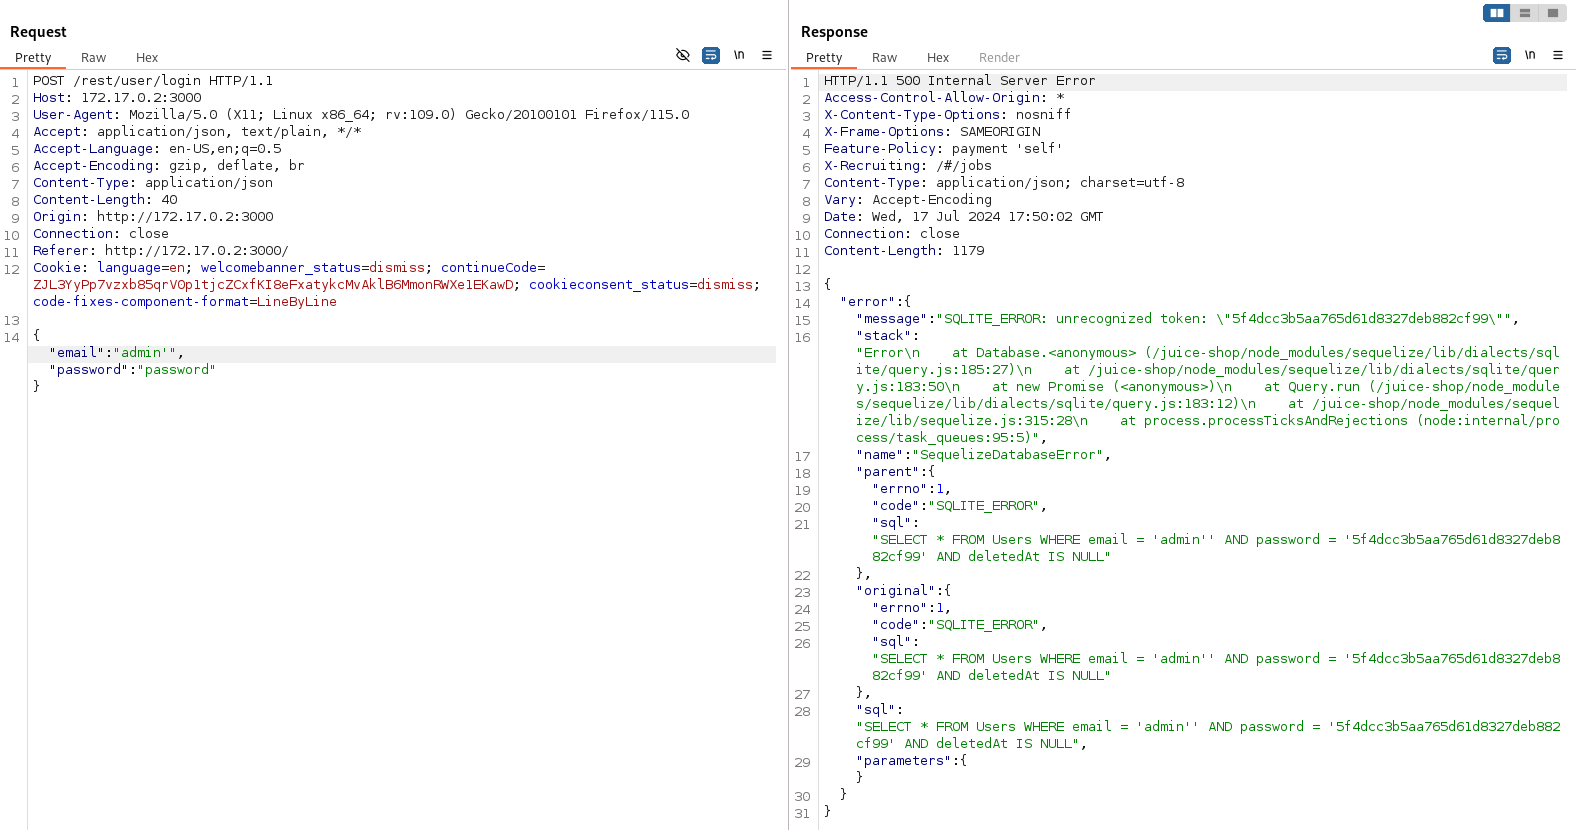
\includegraphics[keepaspectratio]{images/image32.png}}}

{andando a scoprire }{esattamente la query utilizzata e che viene
utilizzato SQLite}{.}

{In questo modo potremmo fare un attacco di tipo }{sql injection}{~per
poter accedere con un account.}

{}

\section{\texorpdfstring{{Exploitation}}{Exploitation}}\label{h.8626r28926e1}

{Tentativi di sfruttamento delle vulnerabilità trovate. }

{}

{Dopo aver riscontrato nella fase precedente che la vulnerabilità nel
login esiste abbiamo }{eseguito un attacco di tipo }{SQL
Injection,}{~andando ad inserire nel campo email:}

{}

{admin' or 1=1 --}

{}

{permettendoci di accedere con l\textquotesingle account admin, questo
perché l'email verrà sempre considerata vera (grazie al 1=1) e la
password verrà saltata, andando a prendere il primo account salvato del
DB.}

{}

{Con questa informazione, e una conoscenza pregressa di SQL, abbiamo
provato a trovare altri account con cui accedere utilizzando un altro
mezzo messo a disposizione da SQL stesso: il }{LIKE}{.}

{Nel dettaglio abbiamo impostato un attacco }{SQL Injection}{~inserendo
nella form:}

{}

{admin' or 1=1 and email not like(`\%admin\%'); --}

{{[}I \% contano come segnaposto all'interno di SQL{]}}

{}

{in questo modo otterremo accesso all'account successivo, che in questo
caso è Jim:}

{\pandocbounded{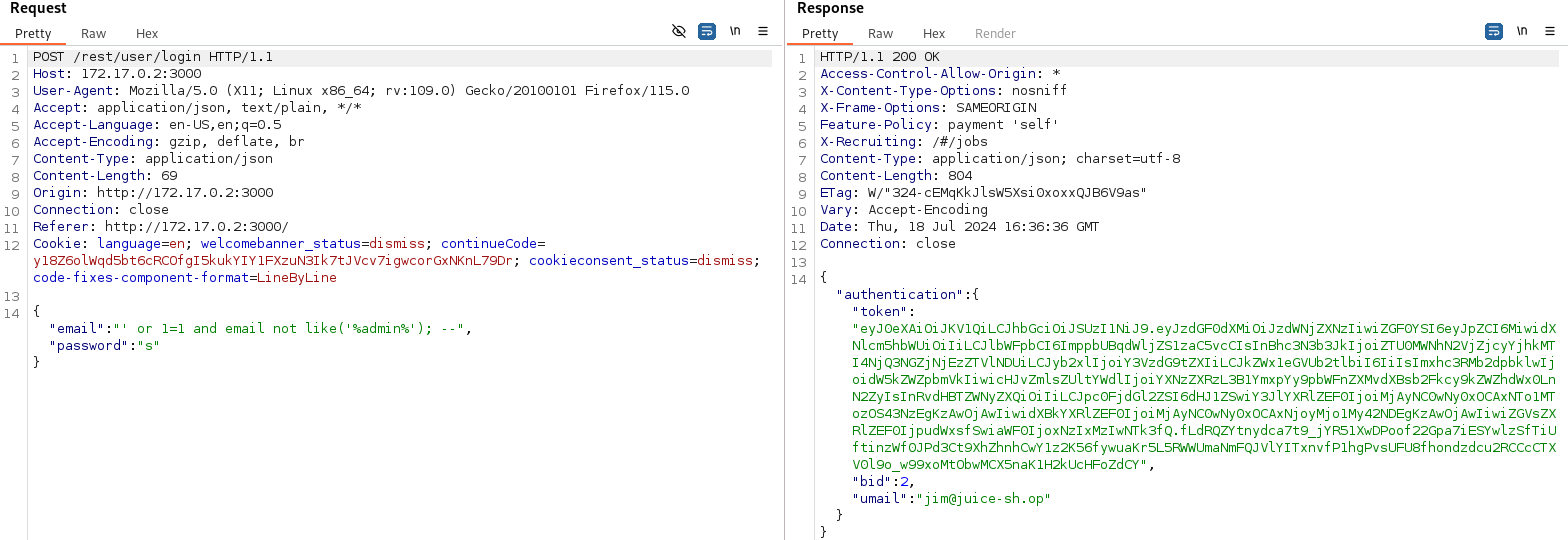
\includegraphics[keepaspectratio]{images/image29.png}}}

{Continuando su questa strada abbiamo fatto:}

{}

{admin' or 1=1 and email not like(`\%admin\%') and email not
like(`\%jim\%'); --}

{}

{ottenendo accesso ad un altro account denominato Bender:}

{\pandocbounded{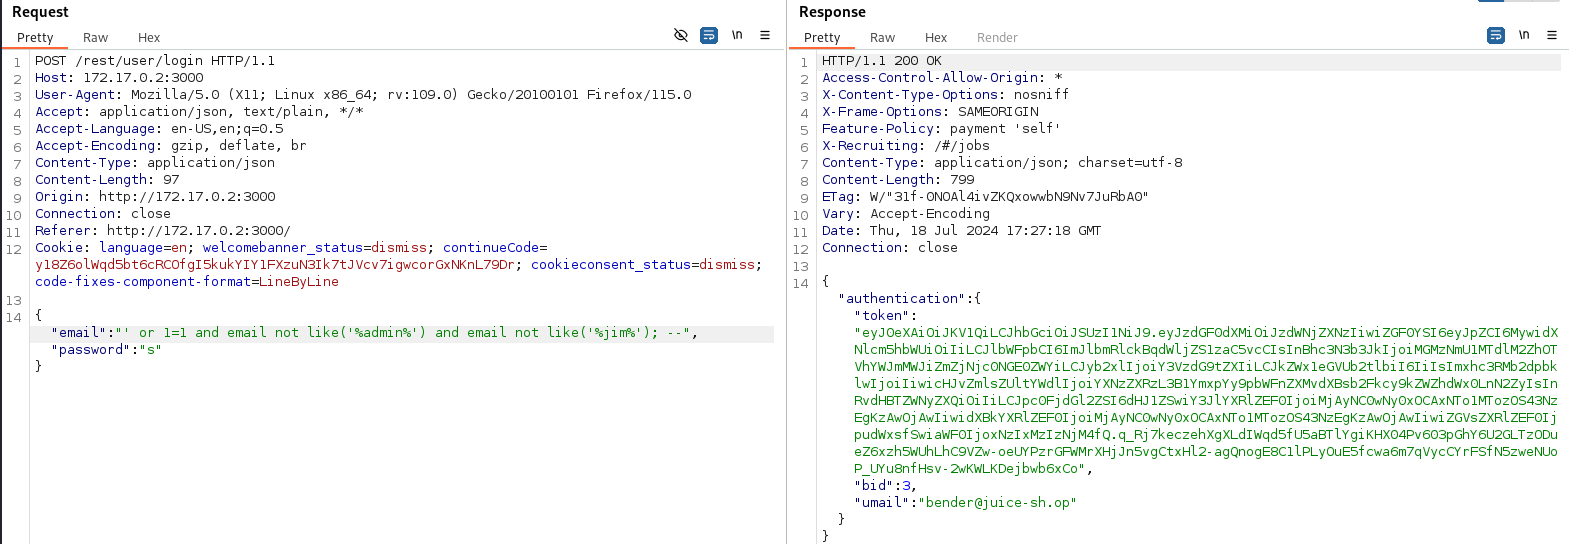
\includegraphics[keepaspectratio]{images/image16.png}}}

{Andando avanti così è possibile accedere a tutti gli account esistenti,
creando non pochi problemi.}

{}

{}

{Ricordandoci dalla fase di information gathering che il sito usa jQuery
versione 2.2.4 sappiamo che è vulnerabile ad attacchi di tipo Cross-site
Scripting (XSS).}

{Tramite questa informazione possiamo provare ad inserire codice
javascript e tag html in tutte quelle parti che accettano input
dall'utente.}

{}

{Se per esempio nella barra di ricerca mettiamo tag html e/o codice
javascript questo viene inserito senza nessun tipo di controllo,
ottenendo questi risultati:}

{\pandocbounded{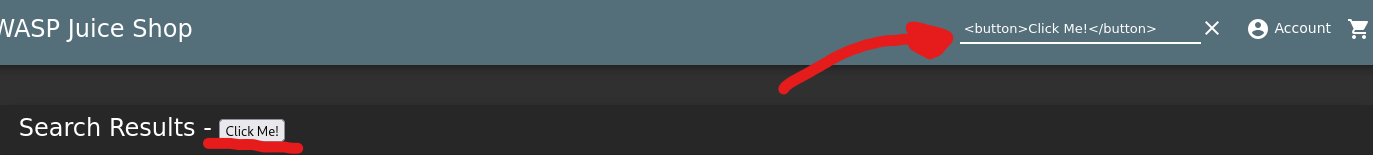
\includegraphics[keepaspectratio]{images/image6.png}}}

{Questo inserendo}{~\textless button\textgreater Click
Me!\textless/button\textgreater{}}{.}

{}

{Oppure inserendo }{\textless iframe src="javascript:alert(`Molto
male\ldots`)"\textgreater{}}{:}

{\pandocbounded{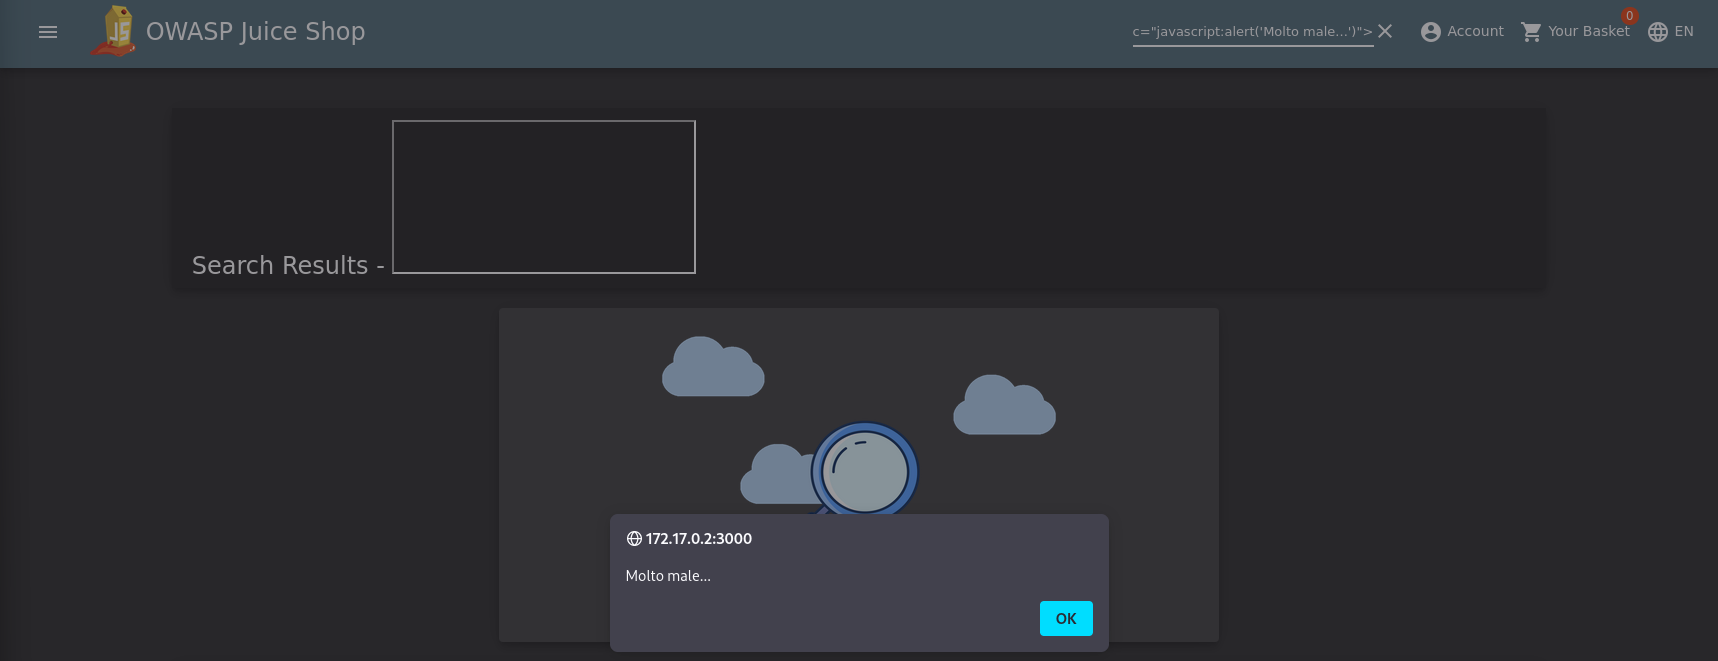
\includegraphics[keepaspectratio]{images/image2.png}}}

{}

\section{\texorpdfstring{{Post-Exploitation}}{Post-Exploitation}}\label{h.539kf6hyfdl6}

{Azioni compiute dopo l\textquotesingle accesso iniziale.}

{}

{Dopo aver ottenuto l'accesso all'account admin siamo andati a
controllare il path trovato nella fase di }{Information Gathering}{,
}{/administration}{, che era inaccessibile senza permessi.}

{}

{In questa sezione possiamo vedere tutti gli account e anche tutte le
recensioni rilasciate, con la possibilità di rimuoverle.}

{\pandocbounded{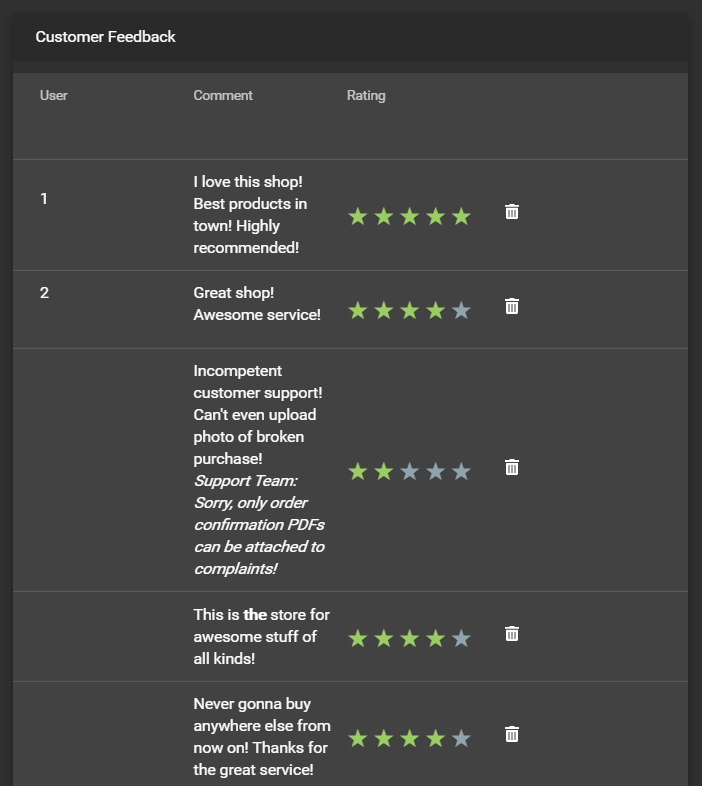
\includegraphics[keepaspectratio]{images/image20.png}}}

{}

{}

{Successivamente abbiamo iniziato a controllare le varie pagine
disponibili solo ad un account registrato.}

{}

{La nostra attenzione è passata subito alla sezione ``}{Your Basket}{'',
che nell'account admin conteneva già dei prodotti: }

{\pandocbounded{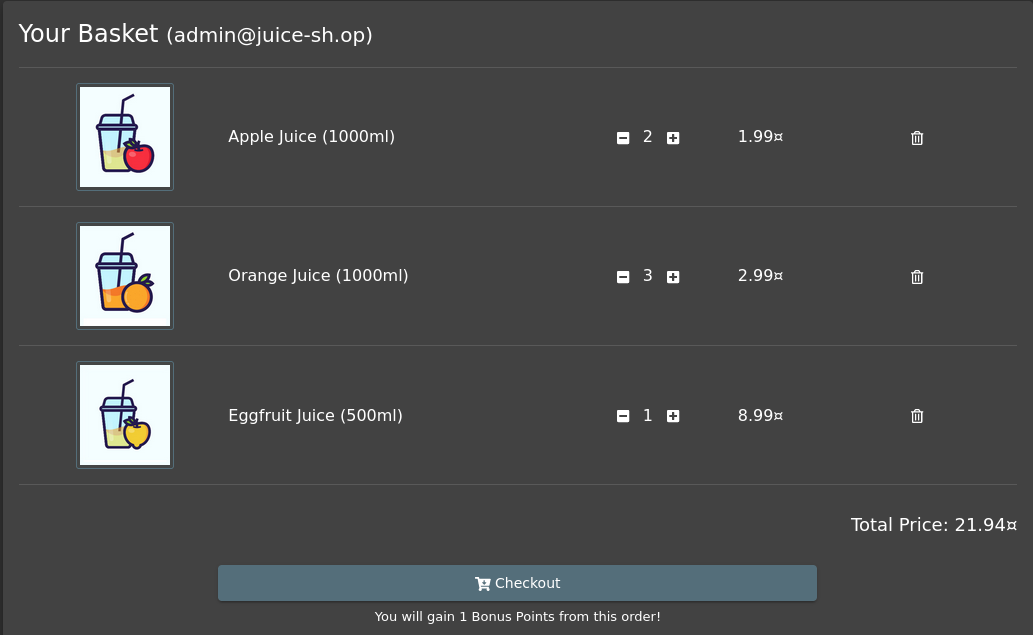
\includegraphics[keepaspectratio]{images/image10.png}}}

{Andando a controllare come questi dati vengono salvati anche alla
chiusura della pagina o al cambio di schermata abbiamo aperto la sezione
Storage nello strumento degli sviluppatori del browser; questo grazie
alle conoscenze pregresse ottenute durante un altro corso, dove abbiamo
creato anche noi una web app per ordinare prodotti.}

{Nello specifico abbiamo controllato il }{Local e Session Storage:}

{\pandocbounded{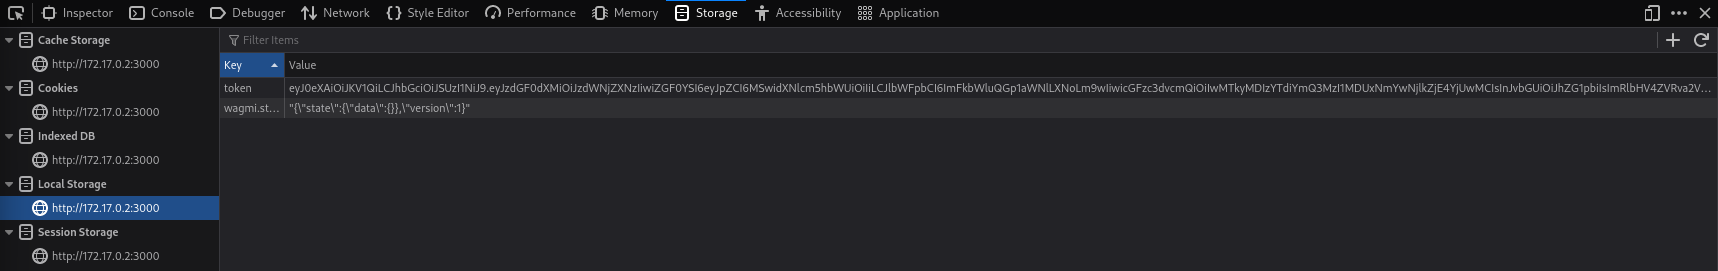
\includegraphics[keepaspectratio]{images/image4.png}}}

{Il }{Local}{~contiene il token di autenticazione.}

{Invece il Session i dettagli del carrello:}

{\pandocbounded{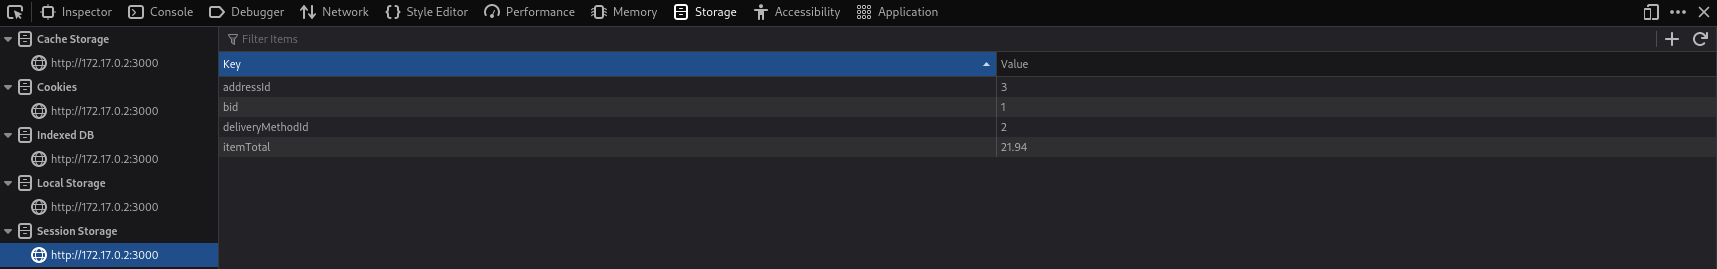
\includegraphics[keepaspectratio]{images/image5.png}}}

{I due valori che ci sono subito caduti sott\textquotesingle occhio sono
il prezzo totale (}{itemTotal}{) e l'id del carrello (}{bid}{). }

{Andando a modificare il primo a 0 per provare a non pagare i prodotti
notiamo, come giusto che sia, che il valore viene
}{ricalcolato}{~rendendo impossibile questo trucco.}

{Modificando invece il }{bid}{~possiamo accedere ad altri carrelli:}

{\pandocbounded{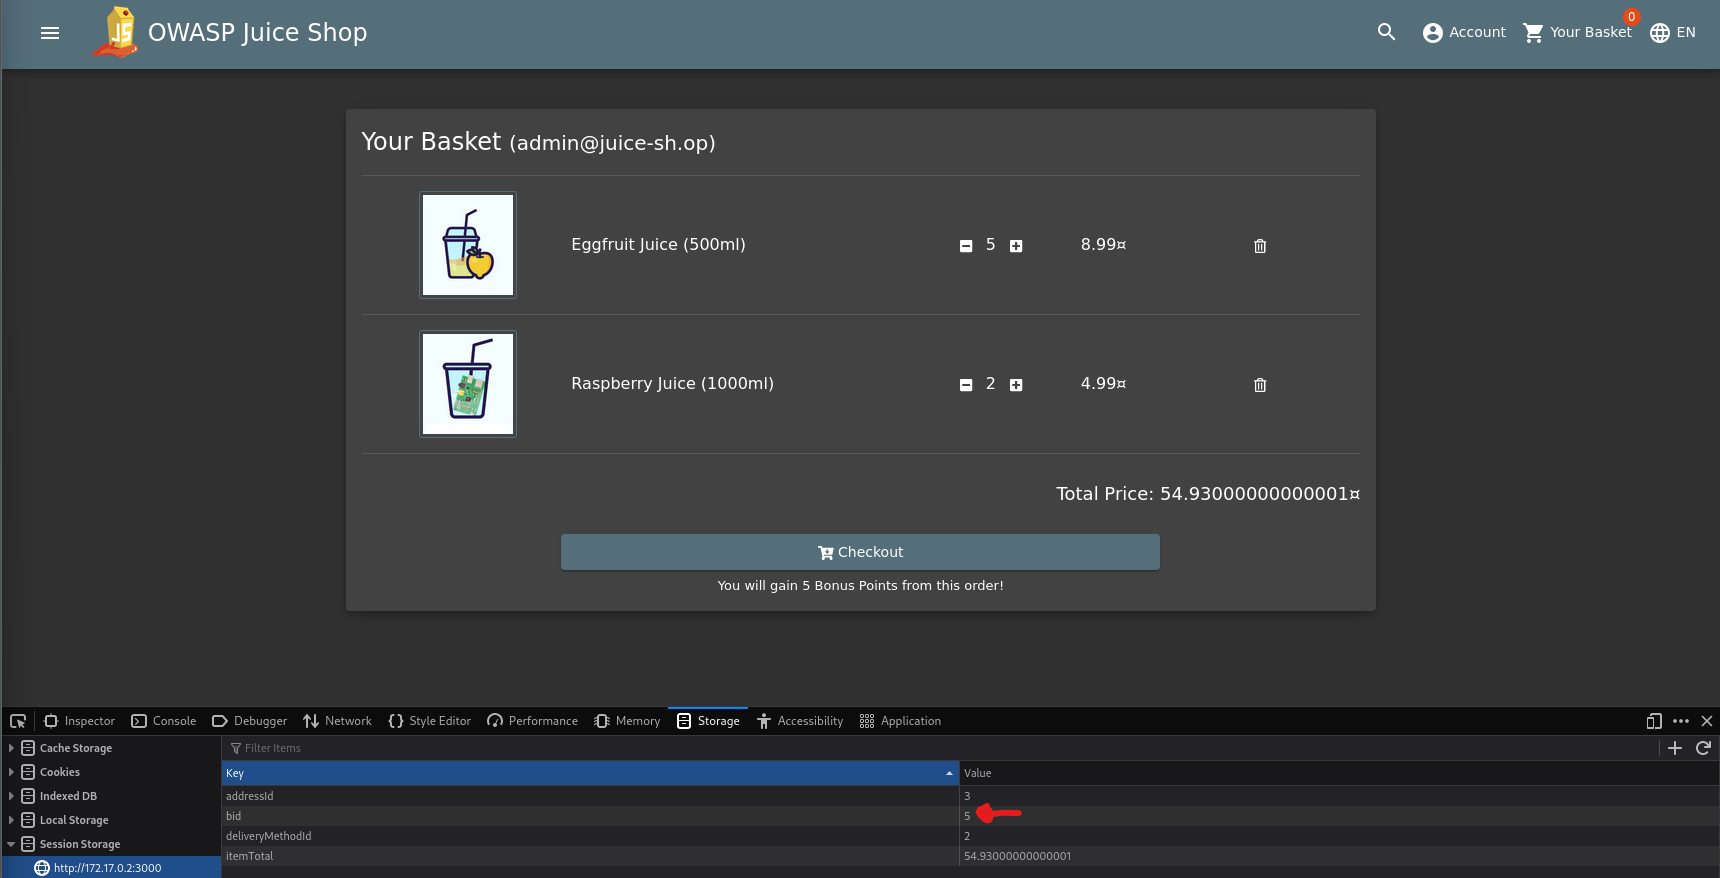
\includegraphics[keepaspectratio]{images/image13.png}}}

{}

{Riuscendo anche a fare il checkout:}

{\pandocbounded{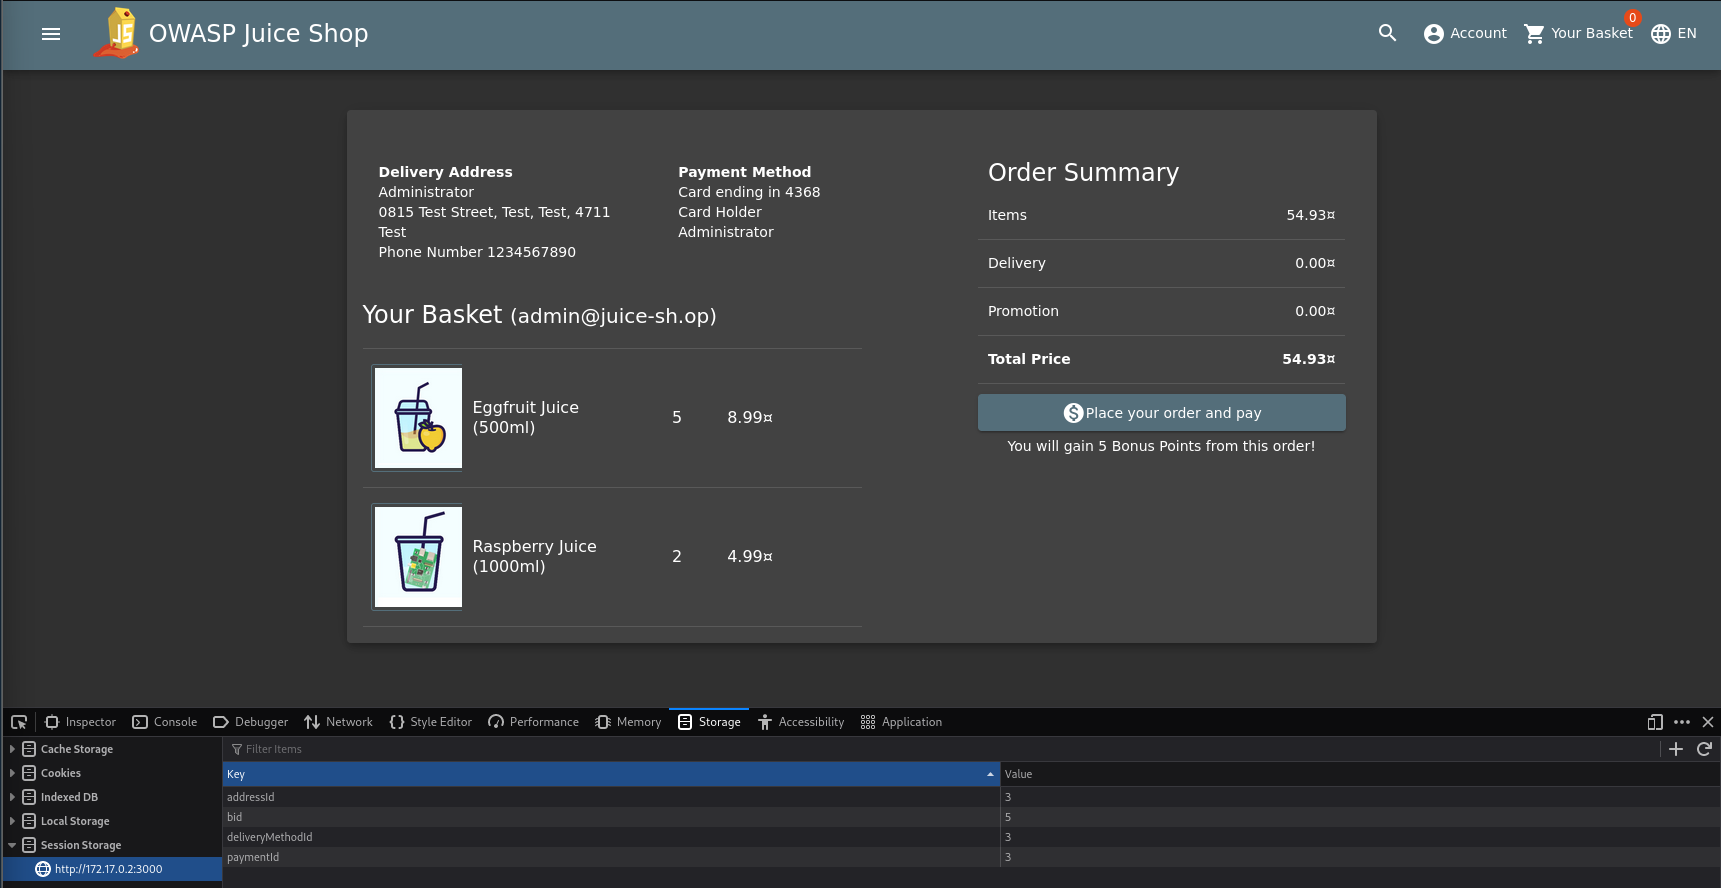
\includegraphics[keepaspectratio]{images/image9.png}}}

{}

{}

{Sapendo dalla fase di Information Gathering che la web app utilizza il
}{``redirect?}{to'' per reindirizzare verso altre pagine, abbiamo deciso
di fare una ricerca all'interno del file }{main.js}{~per trovare tutti
gli utilizzi.}

{Utilizzando il dev tool del browser abbiamo cercato tramite Ctrl+F
tutte le occorrenze del redirect nel file di script, trovando un
redirect che normalmente non sarebbe accessibile.}

{L'URL ritorna a un crypto wallet che probabilmente veniva utilizzato
per ricevere donazioni. ~
~}{\pandocbounded{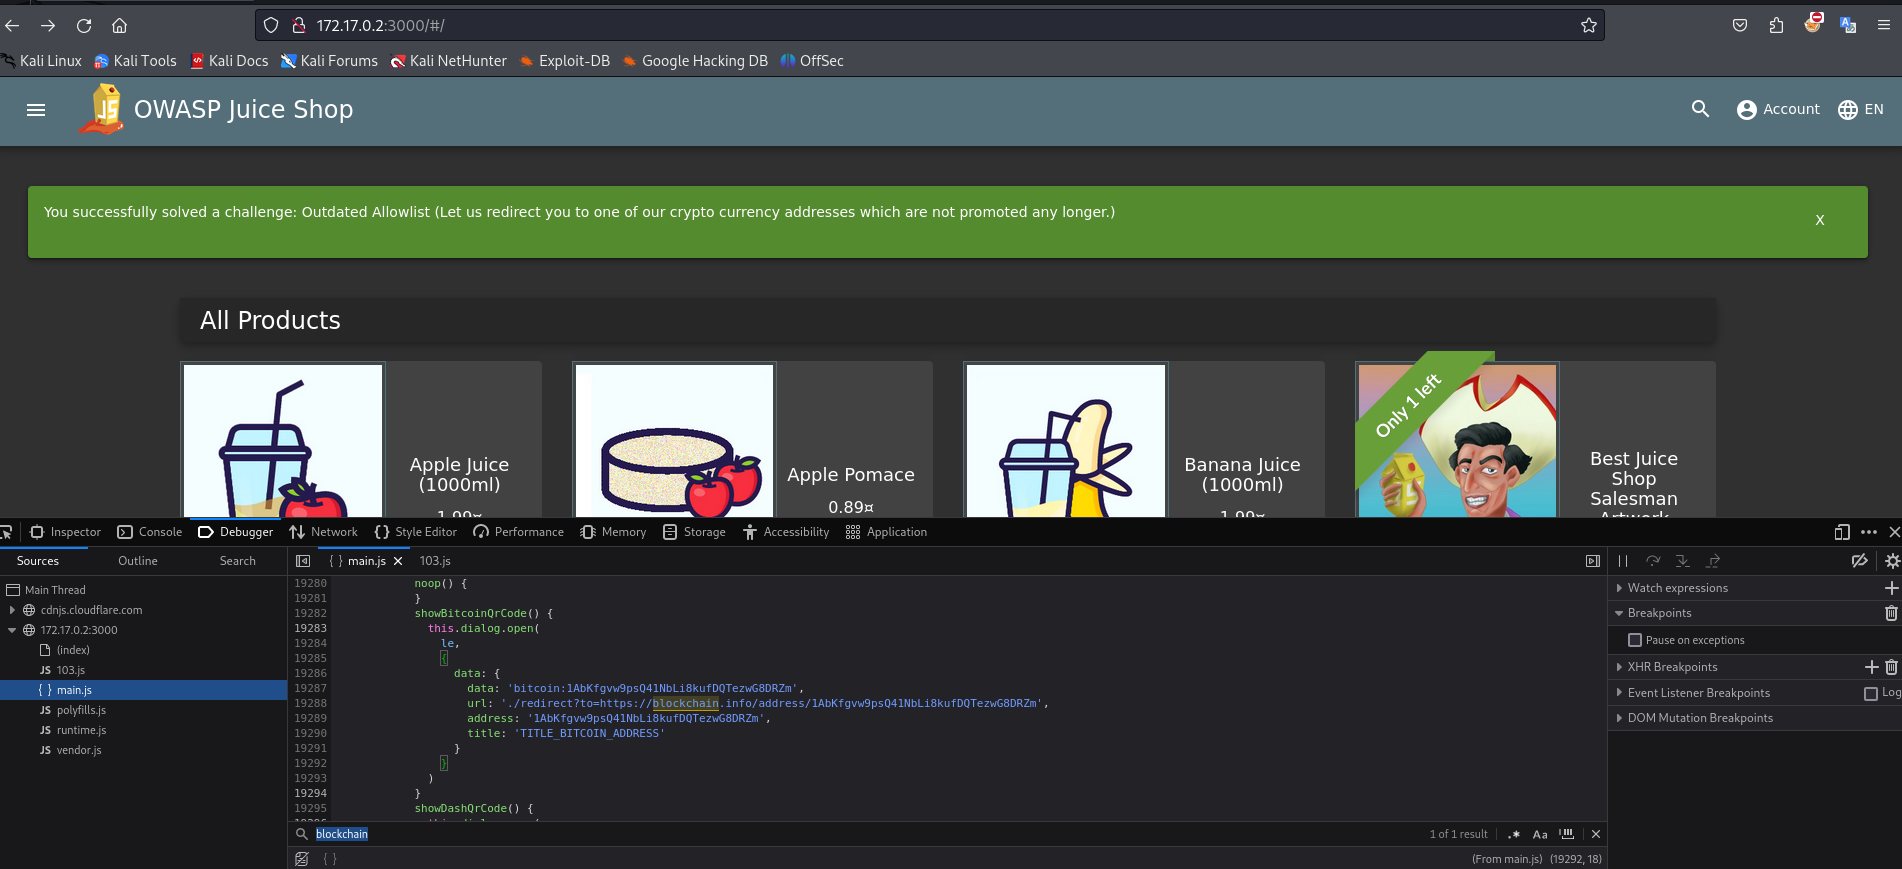
\includegraphics[keepaspectratio]{images/image24.png}}}{~
~}

{}

{Andando a ritroso cercando dove venga utilizzata la funzione
}{showBitcoinQrCode}{~}{possiamo notare che viene chiamata nella parte
di gestione del carrello, ma nella web app non è presente.}

{\pandocbounded{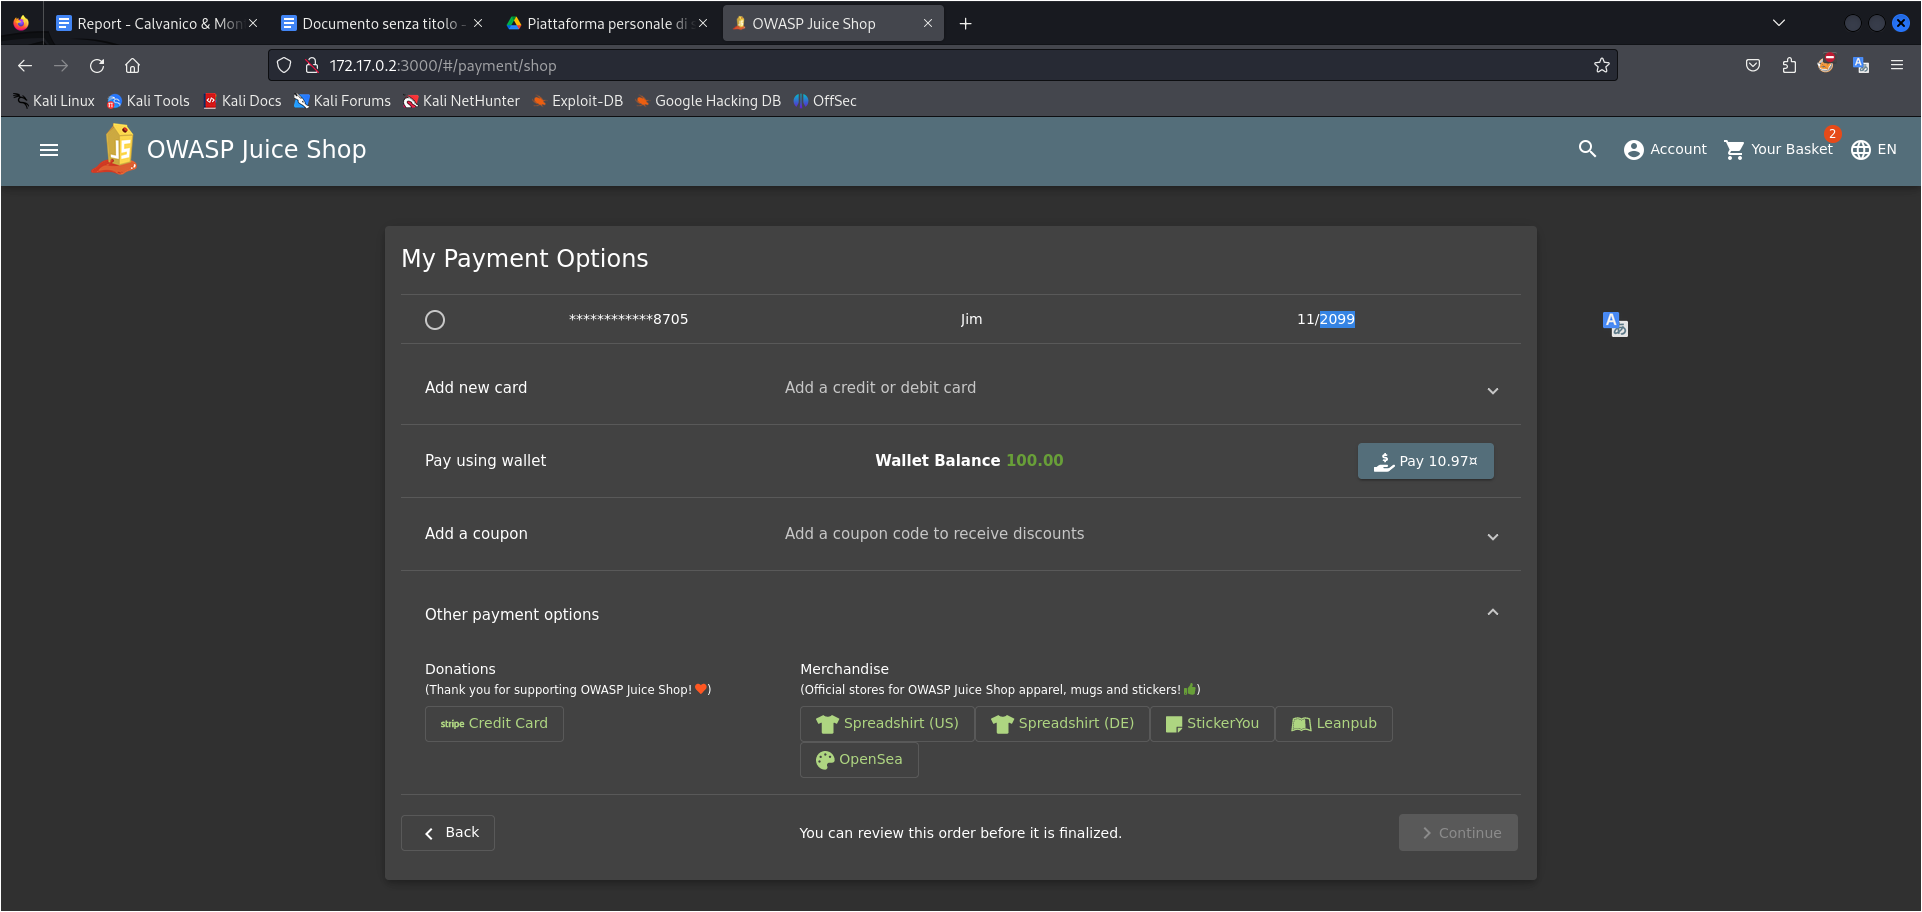
\includegraphics[keepaspectratio]{images/image12.png}}}

{}

{}

{Strumenti Utilizzati}

\section{\texorpdfstring{{Burp
Suite}}{Burp Suite}}\label{h.q6le1yyv8bb0}

\subsection{\texorpdfstring{{Motivo
dell\textquotesingle utilizzo}}{Motivo dell\textquotesingle utilizzo}}\label{h.36laddkt8sd1}

{Lo strumento ci aiuta con un Proxy per intercettare e successivamente
visualizzare le richieste della web app.}

{}

{A differenza degli strumenti degli sviluppatori integrati nel browser,
Burp è più flessibile, permettendo di modificare le richieste,
visualizzarle nella sezione Logger, ecc.}

\subsection{\texorpdfstring{{Obiettivo della
scansione}}{Obiettivo della scansione}}\label{h.pw1vi5mko92c}

{L'obiettivo è cercare nelle richieste informazioni utili per
individuare vulnerabilità ed effettuare exploit. }

\subsection{\texorpdfstring{{Spiegazione del
funzionamento}}{Spiegazione del funzionamento}}\label{h.pr2ckmjmbrp8}

{Burp intercetta e blocca le richieste verso e da la web app, questo è
possibile perché abbiamo installato un\textquotesingle estensione nel
browser utilizzato (FireFox), chiamata FoxyProxy, che implementa un
proxy che }{ri-indirizza}{~le richieste verso Burp permettendoci di
interagire con esse.}

{\pandocbounded{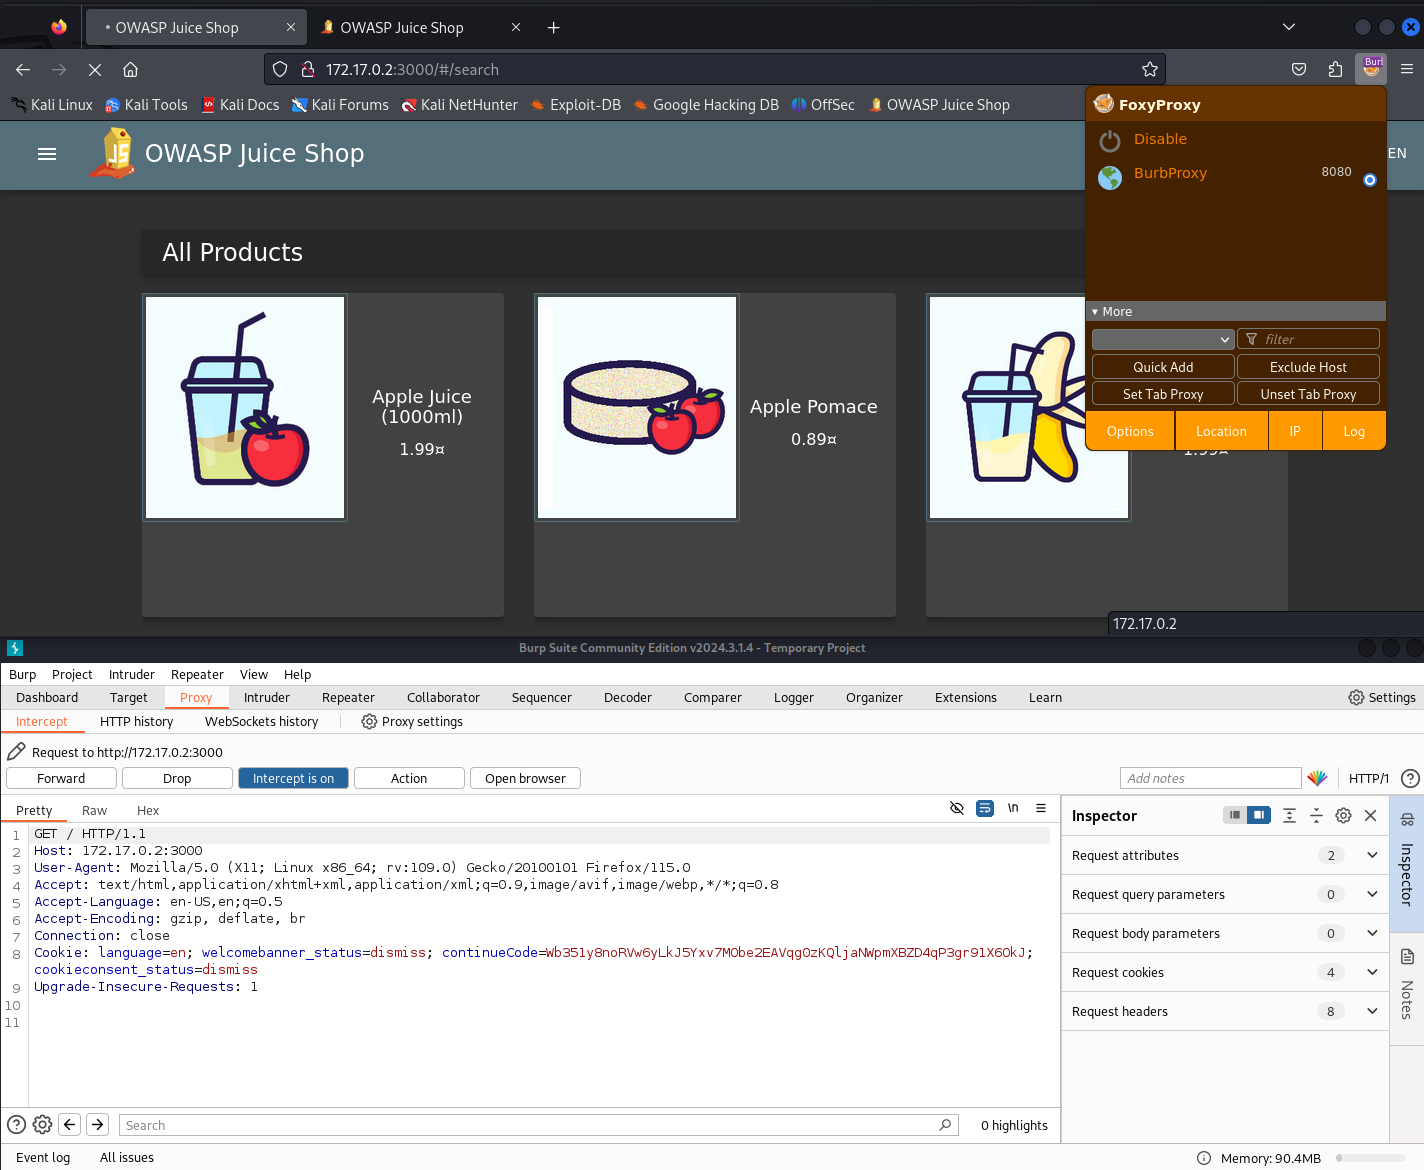
\includegraphics[keepaspectratio]{images/image14.png}}}

{}

\section{\texorpdfstring{{Nmap}}{Nmap}}\label{h.dzuh2av1ipln}

\subsection{\texorpdfstring{{Motivo
dell\textquotesingle utilizzo}}{Motivo dell\textquotesingle utilizzo}}\label{h.f09udkfoe018}

{Utilizzato per fare service enumeration, specifichiamo }{l'ip +
porta}{~e il tool ci restituisce i servizi, con rispettive versioni
utilizzate.}

\subsection{\texorpdfstring{{Obiettivo della
scansione}}{Obiettivo della scansione}}\label{h.w68y2kll35ri}

{Scoprire che servizi vengono utilizzati dalla web app con anche la
versione per cercare possibili vulnerabilità.}

\subsection{\texorpdfstring{{Spiegazione del
funzionamento}}{Spiegazione del funzionamento}}\label{h.uy9oh1cg3sub}

{Tramite comando:}

{nmap -p{[}PORT{]} {[}FLAG{]} {[}IP{]}}

{}

{il tool invia pacchetti al host e in base alla risposta capisce se una
porta è aperta, filtrata o chiusa e quindi se un servizio è utilizzato o
meno oppure può ottenere informazioni sul OS.}

{}

\section{\texorpdfstring{{Wappalyzer}}{Wappalyzer}}\label{h.boxe1ftvjrr}

\subsection{\texorpdfstring{{Motivo
dell\textquotesingle utilizzo}}{Motivo dell\textquotesingle utilizzo}}\label{h.dtueno752xs8}

{Utilizzato per ottenere informazioni sulle tecnologie utilizzate dal
sito e relative versioni}

\subsection{\texorpdfstring{{Obiettivo della
scansione}}{Obiettivo della scansione}}\label{h.6k40l5sirmys}

{Trovare tecnologie vulnerabili nella web app in modo da fare l'exploit
su di esse.}

\subsection{\texorpdfstring{{Spiegazione del
funzionamento}}{Spiegazione del funzionamento}}\label{h.dl2s5hs3ttbs}

{il tool cerca negli header http, nel codice html e script informazioni
che potrebbero }{ritornare}{~a certe tecnologie e versioni.}

{}

\section{\texorpdfstring{{WAF00F}}{WAF00F}}\label{h.ugp6xcvx77ev}

\subsection{\texorpdfstring{{Motivo
dell\textquotesingle utilizzo}}{Motivo dell\textquotesingle utilizzo}}\label{h.y5oaetewmvgs}

{Tool perfetto per controllare la presenza di WAF in maniera veloce e
senza troppe configurazioni.}

\subsection{\texorpdfstring{{Obiettivo della
scansione}}{Obiettivo della scansione}}\label{h.mmz6tca61ulu}

{Trovare che tipo di WAF viene usato in modo da sapere quale tipo di
traffico viene bloccato o meno, utile per usare certi exploit.}

\subsection{\texorpdfstring{{Spiegazione del
funzionamento}}{Spiegazione del funzionamento}}\label{h.1p6jyw29r7y3}

{Tramite comando:}

{waf00f {[}INDIRIZZO{]}}

{}

{invia una serie di richieste HTTP a un sito web e analizza le risposte
per identificare il WAF in uso.}

{}

\section{\texorpdfstring{{Wireshark}}{Wireshark}}\label{h.n379yqkt947w}

\subsection{\texorpdfstring{{Motivo
dell\textquotesingle utilizzo}}{Motivo dell\textquotesingle utilizzo}}\label{h.grnxuxqwt1j5}

{Fare lo sniff dei pacchetti HTTP verso e dalla web app.}

\subsection{\texorpdfstring{{Obiettivo della
scansione}}{Obiettivo della scansione}}\label{h.x3c31ml4fogs}

{Prova manuale per avere un\textquotesingle ulteriore conferma che le
risposte HTTP non vengano alterate da uno strumento di
detection/response.}

\subsection{\texorpdfstring{{Spiegazione del
funzionamento}}{Spiegazione del funzionamento}}\label{h.4wk6nd6xtx0s}

{Il tool intercetta i pacchetti in arrivo e verso un obiettivo con la
possibilità di filtrarli.}

{}

\section{\texorpdfstring{{Nikto}}{Nikto}}\label{h.3scydxz736u}

\subsection{\texorpdfstring{{Motivo
dell\textquotesingle utilizzo}}{Motivo dell\textquotesingle utilizzo}}\label{h.pk65094qd1ba}

{Come automatic scanners è veloce e applicabile a qualsiasi realtà.}

\subsection{\texorpdfstring{{Obiettivo della
scansione}}{Obiettivo della scansione}}\label{h.v8e13aujp8bs}

{Trovare path che non dovrebbero essere accessibili dagli utenti in modo
da scovare informazioni sensibili.}

\subsection{\texorpdfstring{{Spiegazione del
funzionamento}}{Spiegazione del funzionamento}}\label{h.me4nvlhmahdn}

{Tramite comando:}

{nikto -host{[}INDIRIZZO{]}}

{}

{il tool ricerca informazioni sul web server o
sull\textquotesingle applicazione web da
}{scansionare;}{~successivamente inizia la scansione utilizzando
richieste http e file.}

\section{\texorpdfstring{{FFUF}}{FFUF}}\label{h.sqt62nmz4moo}

\subsection{\texorpdfstring{{Motivo
dell\textquotesingle utilizzo}}{Motivo dell\textquotesingle utilizzo}}\label{h.9x6besqrxucw}

{Abbiamo scelto questo tool invece che altri, con lo stesso scopo,
perché più veloce e con tanti flag utili per personalizzare la ricerca.}

\subsection{\texorpdfstring{{Obiettivo della
scansione}}{Obiettivo della scansione}}\label{h.t277em3zvhs1}

{Trovare nuove sottodirectory per scovare vulnerabilità o tecnologie
usate dalla web app.}

\subsection{\texorpdfstring{{Spiegazione del
funzionamento}}{Spiegazione del funzionamento}}\label{h.fwcmrnwiwxed}

{Tramite comando:}

{ffuf}{~}{-u{[}INDIRIZZO{]}}{~-w{[}PATH WORDLIST{]} ~-fs{[}SIZE
RISPOSTA{]}}

{}

{il tool parte dal rootdir e ricerca ricorsivamente su ogni
sottodirectory trovata; i due flag utilizzati fanno:}

\begin{itemize}
\tightlist
\item
  {-w}{: prende una wordlist dal path inserito;}
\item
  {-fs}{: filtra le risposte in base al size del ritorno, ci è servito
  perché la webapp in caso di indirizzo errato ritorna la pagina
  iniziale.}
\end{itemize}

{}

{}

{Analisi delle Vulnerabilità }

\section{\texorpdfstring{{SQL Injection -
Login}}{SQL Injection - Login}}\label{h.hanyn33oswiy}

\subsection{\texorpdfstring{{Descrizione della
vulnerabilità}}{Descrizione della vulnerabilità}}\label{h.wlp9x9bbg7lc}

{Tramite l'inserimento di certi caratteri e stringhe tipiche di SQL, e
inaspettati dal server, è possibile eseguire codice malevolo.}

{}

{In questo caso usata per ottenere accesso ad uno o più account (tra cui
quello dell'admin).}

\subsection{\texorpdfstring{{Riproducibilità}}{Riproducibilità}}\label{h.fqeix86gxey}

{Per riprodurre la vulnerabilità bisogna:}

\begin{enumerate}
\tightlist
\item
  {andare nella pagine di login;}
\item
  {inserire la seguente stringa }{nell'email:}{~}{Placeholder' or 1=1
  --}{;}
\item
  {inserire qualunque cosa nella password;}
\item
  {cliccare invio.}
\end{enumerate}

{}

{In sostanza va messo dopo l'or una condizione sempre vera, seguito dai
simboli per commentare.}

\subsection{\texorpdfstring{{Prova della
rilevazione}}{Prova della rilevazione}}\label{h.s0jebivrvcpy}

{\pandocbounded{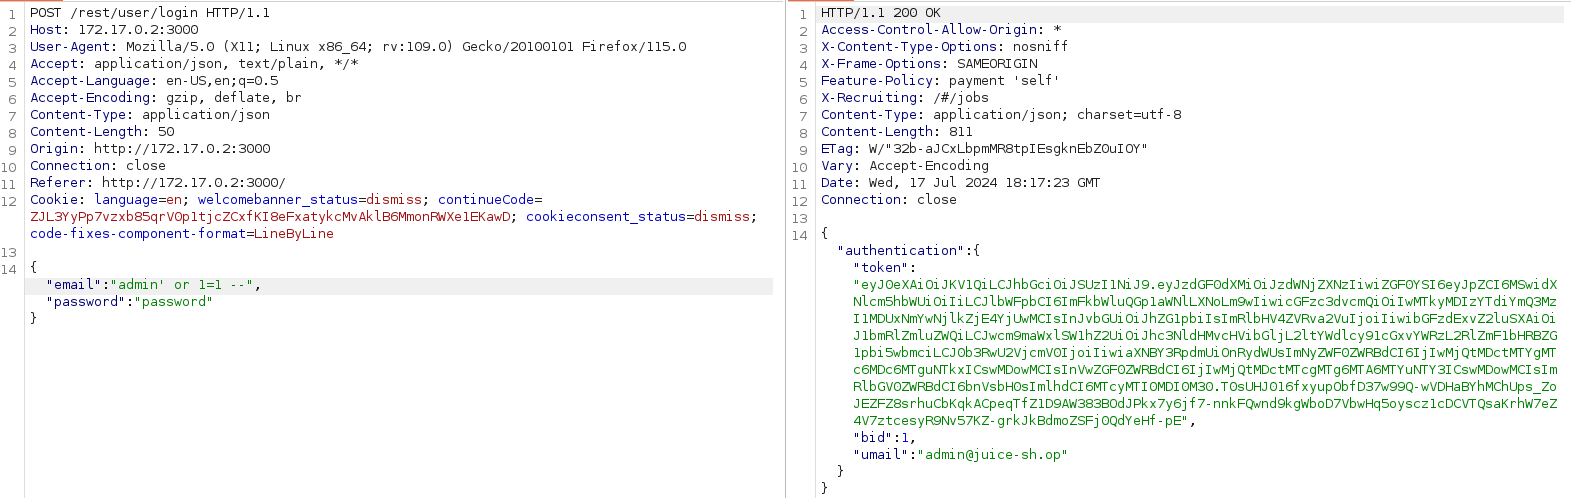
\includegraphics[keepaspectratio]{images/image19.png}}}

\subsection{\texorpdfstring{{Classificazione OWASP TOP
10}}{Classificazione OWASP TOP 10}}\label{h.yawlloeej79a}

{Secondo }{l'OWASP}{~questo tipo di vulnerabilità è classificata:}

{\pandocbounded{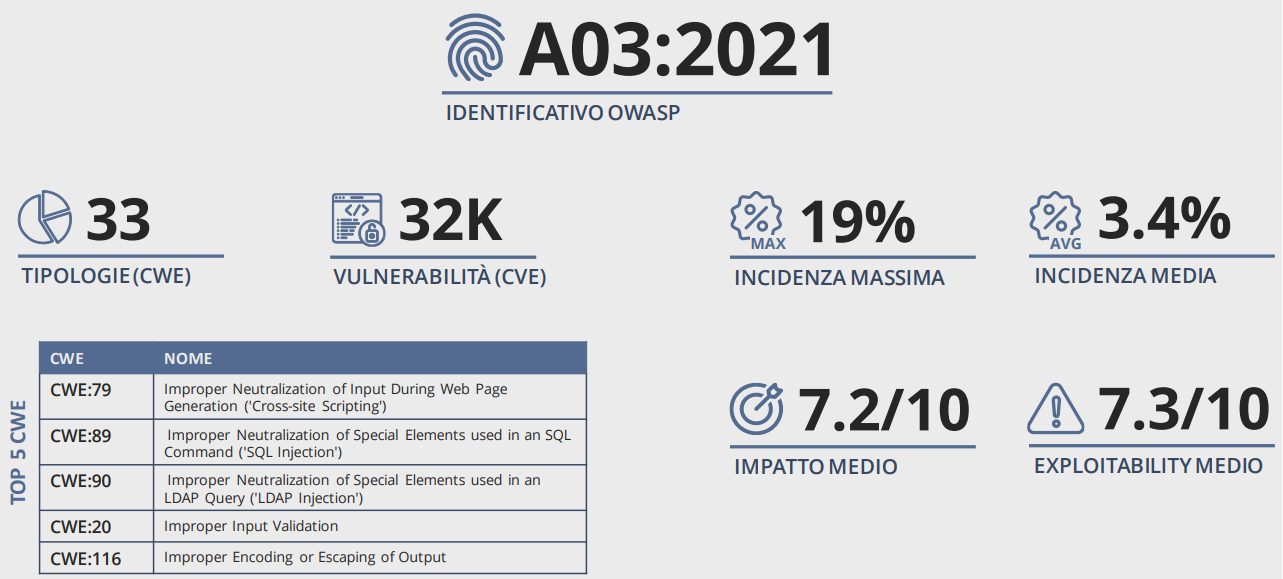
\includegraphics[keepaspectratio]{images/image11.png}}}

{}

{Lo score del CVSS è:}

{\pandocbounded{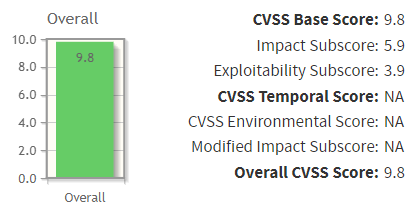
\includegraphics[keepaspectratio]{images/image23.png}}}

{Con le seguente metriche:}

{\pandocbounded{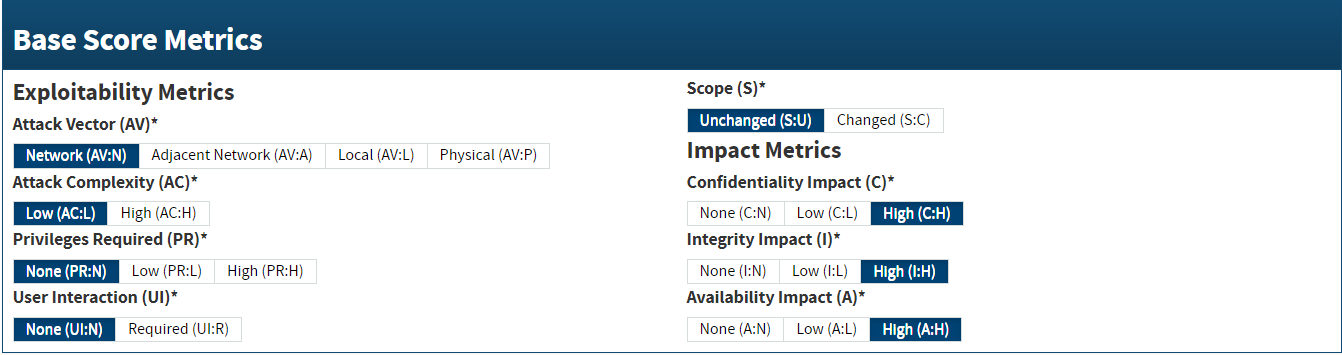
\includegraphics[keepaspectratio]{images/image8.png}}}

\subsection{\texorpdfstring{{Requisiti
dell\textquotesingle attaccante}}{Requisiti dell\textquotesingle attaccante}}\label{h.8d2l9necu0xo}

{L'unica cosa necessaria è avere accesso al sito web e una conoscenza di
SQL.}

\subsection{\texorpdfstring{{Gravità e
Impatti}}{Gravità e Impatti}}\label{h.hmp3fn5snz93}

{Questa vulnerabilità è estremamente grave, perché permette di accedere
come admin all'applicativo web con un impatto non indifferente
sull'integrità dell'applicativo e dei dati. }

{}

\section{\texorpdfstring{{XSS - DOM}}{XSS - DOM}}\label{h.hkn8w3frpte2}

\subsection{\texorpdfstring{{Descrizione della
vulnerabilità}}{Descrizione della vulnerabilità}}\label{h.u2qilstmcadt}

{Un Cross-Site Scripting è una vulnerabilità che permette a un
malintenzionato di iniettare codice dannoso all\textquotesingle interno
di un sito web legittimo.}

\subsection{\texorpdfstring{{Riproducibilità}}{Riproducibilità}}\label{h.dbaegubiyg2}

{Nel nostro caso tramite il campo ricerca siamo riusciti ad inserire nel
DOM componenti HTML, come bottoni e alert, ecco gli step:}

\begin{enumerate}
\tightlist
\item
  {aprire il campo ricerca;}
\item
  {inserire qualunque tag si voglia, nel nostro caso: }{\textless iframe
  src="javascript:alert(`Molto male\ldots`)"\textgreater{}}{;}
\item
  {all'invio si vedrà nel DOM della pagina il tag inserito nel campo di
  input.}
\end{enumerate}

\subsection{\texorpdfstring{{Prova della
rilevazione}}{Prova della rilevazione}}\label{h.zcsbwhbzmg7u}

{\pandocbounded{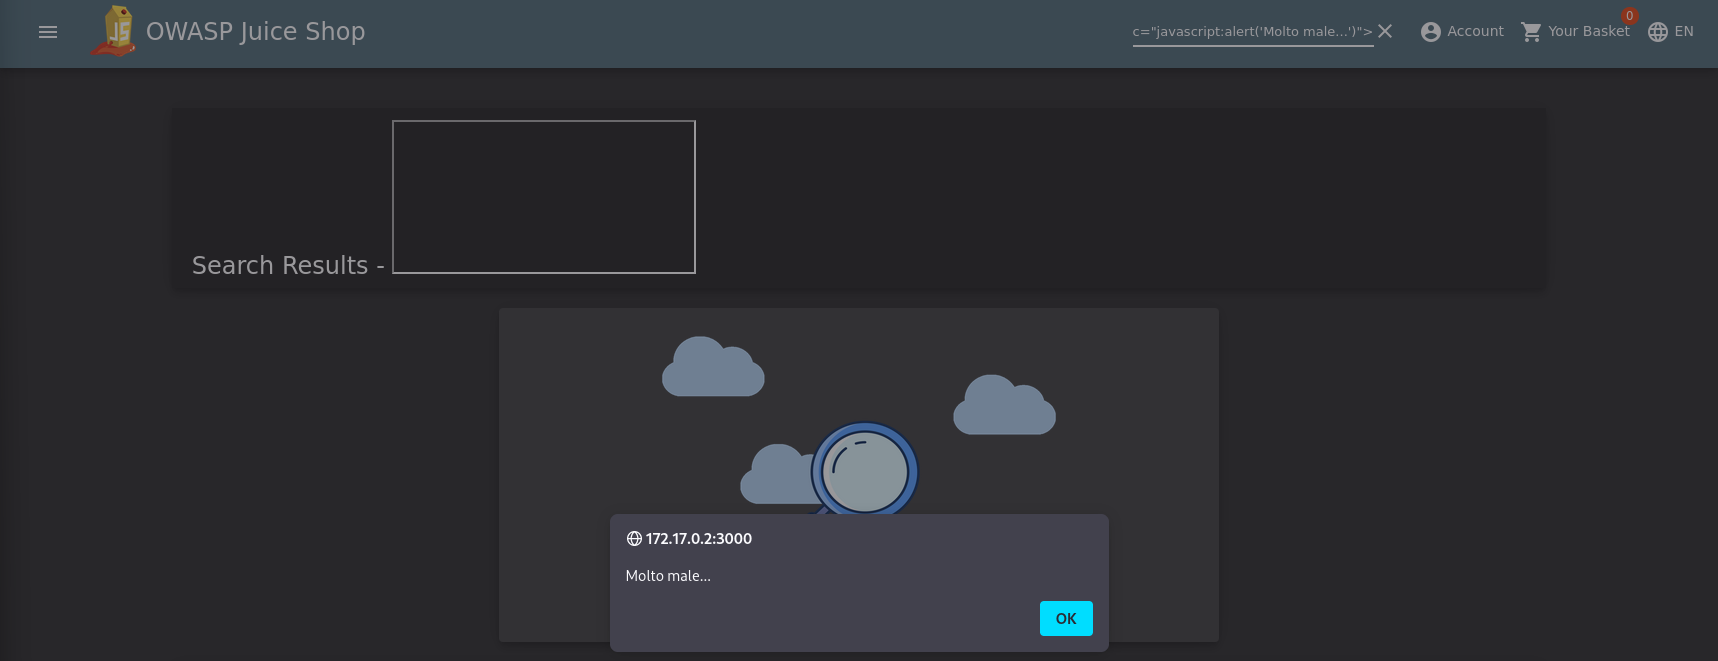
\includegraphics[keepaspectratio]{images/image2.png}}}

\subsection{\texorpdfstring{{Classificazione OWASP TOP
10}}{Classificazione OWASP TOP 10}}\label{h.akjclfce3m3t}

{Secondo }{l'OWASP}{~questo tipo di vulnerabilità è classificata:}

{\pandocbounded{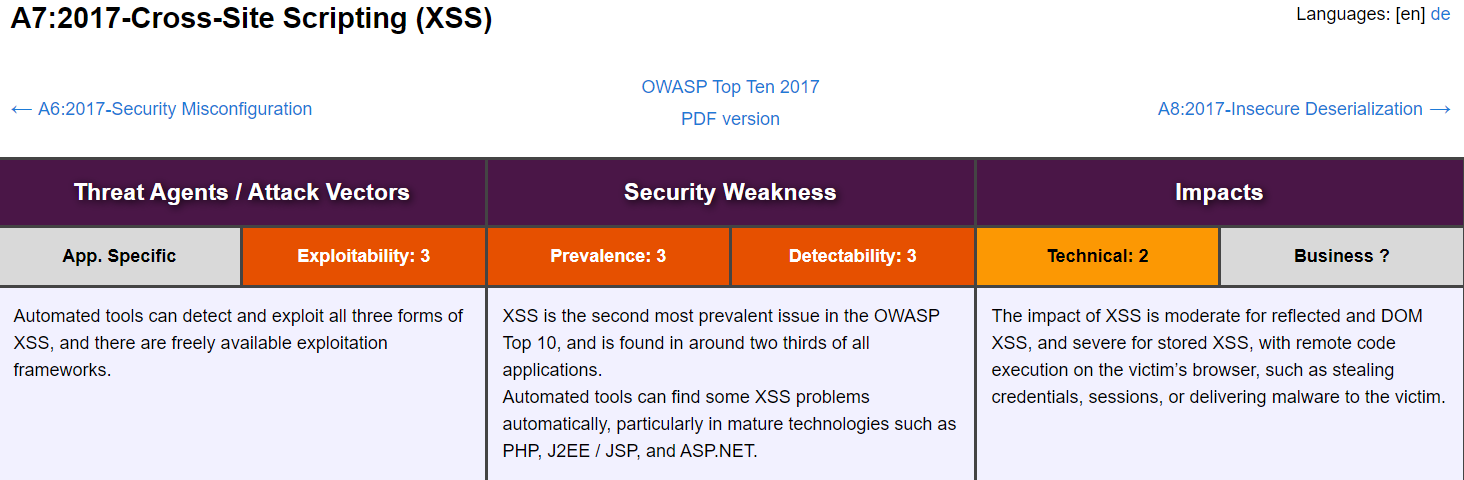
\includegraphics[keepaspectratio]{images/image7.png}}}

{}

{Lo score del CVSS è:}

{\pandocbounded{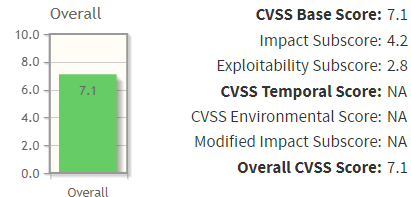
\includegraphics[keepaspectratio]{images/image30.png}}}

{Con le seguente metriche:}

{\pandocbounded{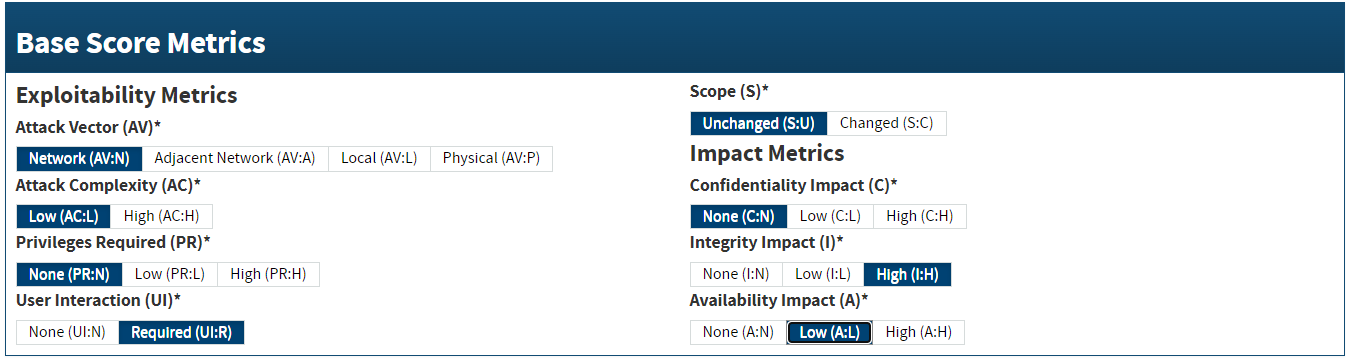
\includegraphics[keepaspectratio]{images/image26.png}}}

{}

\subsection{\texorpdfstring{{Requisiti
dell\textquotesingle attaccante}}{Requisiti dell\textquotesingle attaccante}}\label{h.chbz8re57zbj}

{L'attaccante deve solo aver accesso alla web app e conoscere un minimo
di html.}

\subsection{\texorpdfstring{{Gravità e
Impatti}}{Gravità e Impatti}}\label{h.hv0rtn93md00}

{Se la modifica, che viene fatta tramite questa vulnerabilità, rimane
salvata all'interno della pagina il codice javascript verrà eseguito sul
browser dell'utente ad ogni accesso, creando situazioni altamente
pericolose.}

{}

{La vulnerabilità ha una gravità moderata se il codice non viene salvato
(}{Reflected XSS}{) con impatti medio/bassi, al contrario si ha una
gravità e un impatto critici.}

{}

\section{\texorpdfstring{{Broken Access }{Control}{~- Accesso ad un
altro
carrello}}{Broken Access Control~- Accesso ad un altro carrello}}\label{h.jtzze9vhb77t}

\subsection{\texorpdfstring{{Descrizione della
vulnerabilità}}{Descrizione della vulnerabilità}}\label{h.ymnlgohc8kto}

{Tramite una configurazione errata del }{Session Storage}{~e dei
permessi è possibile accedere al carrello di un altro utente, con la
possibilità di effettuare tutte le normali attività.}

\subsection{\texorpdfstring{{Riproducibilità}}{Riproducibilità}}\label{h.541z6ku05wnf}

{Per effettuare questa vulnerabilità è necessario:}

\begin{enumerate}
\tightlist
\item
  {essere autenticati ad un account;}
\item
  {aprire il carrello e il dev tool del browser;}
\item
  {nella sezione }{Session Storage}{~cambiare il campo }{bid}
\end{enumerate}

\subsection{\texorpdfstring{{Prova della
rilevazione}}{Prova della rilevazione}}\label{h.vmjkki6ithr3}

{Bid prima del cambio:}

{\pandocbounded{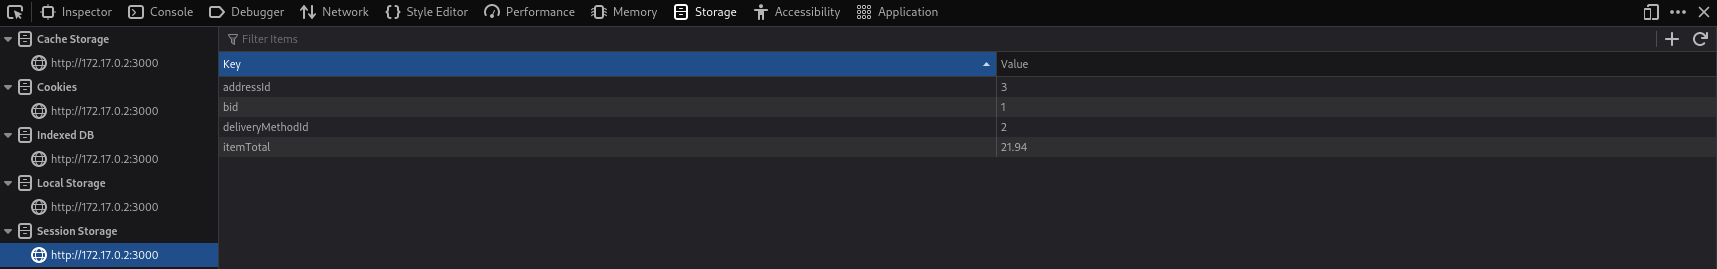
\includegraphics[keepaspectratio]{images/image5.png}}}

{}

{Bid e carrello dopo il cambio:}

{\pandocbounded{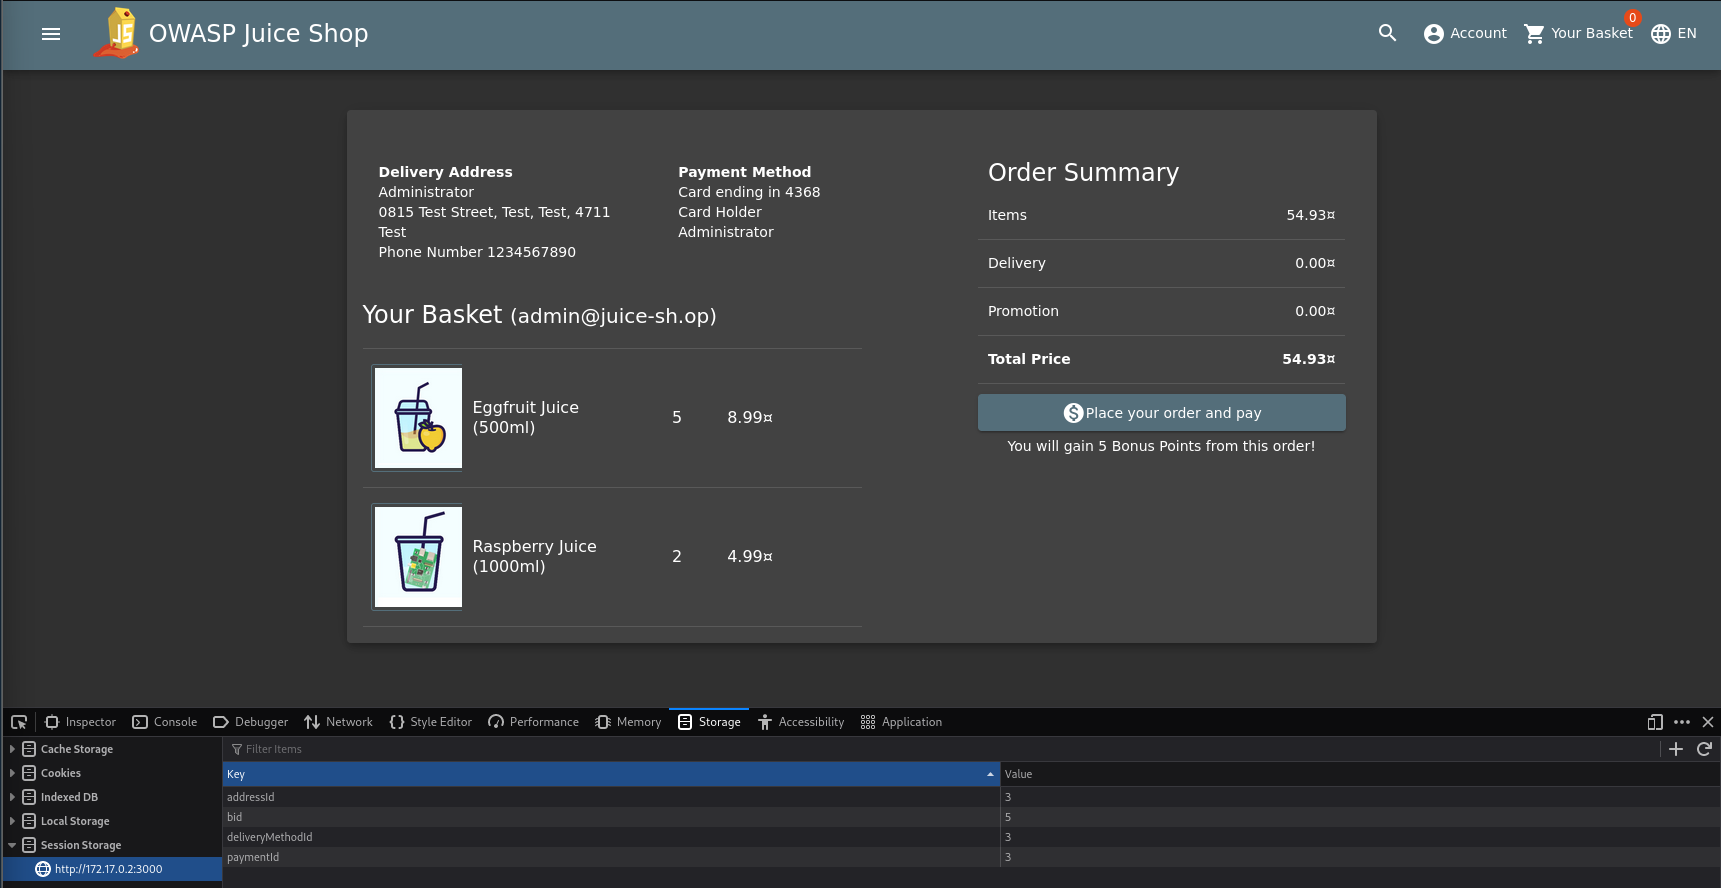
\includegraphics[keepaspectratio]{images/image9.png}}}

\subsection{\texorpdfstring{{Classificazione OWASP TOP
10}}{Classificazione OWASP TOP 10}}\label{h.puapvvc1zkco}

{Secondo }{l'OWASP}{~questo tipo di vulnerabilità è classificata:}

{\pandocbounded{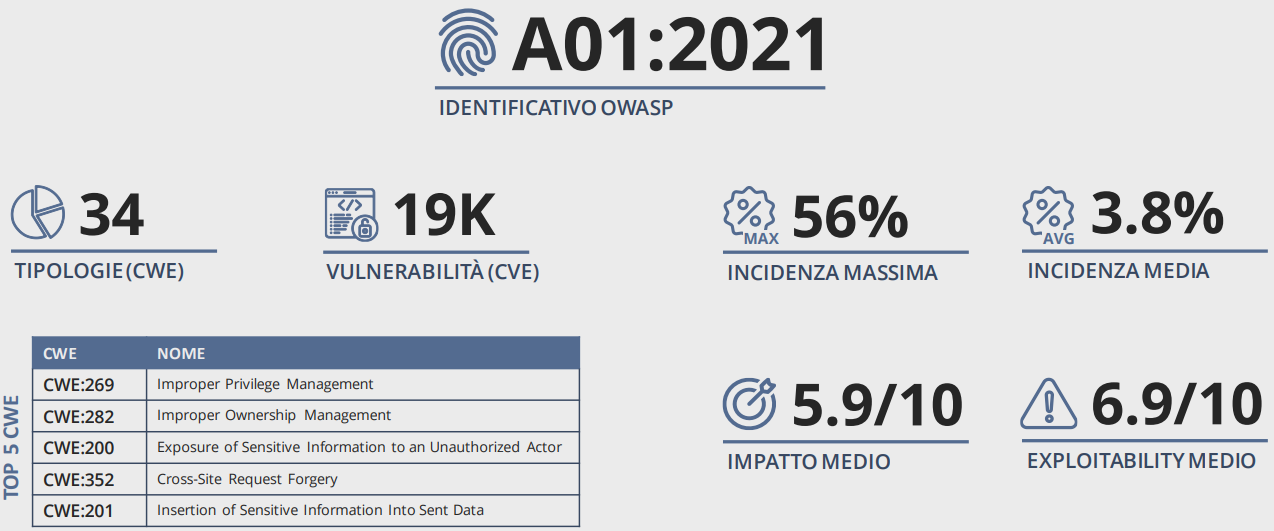
\includegraphics[keepaspectratio]{images/image18.png}}}

{}

{Lo score del CVSS è:}

{\pandocbounded{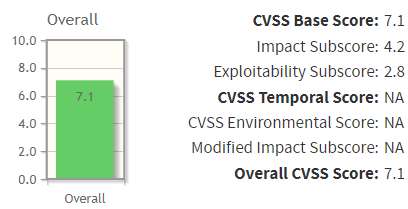
\includegraphics[keepaspectratio]{images/image27.png}}}

{Con le seguente metriche:}

{\pandocbounded{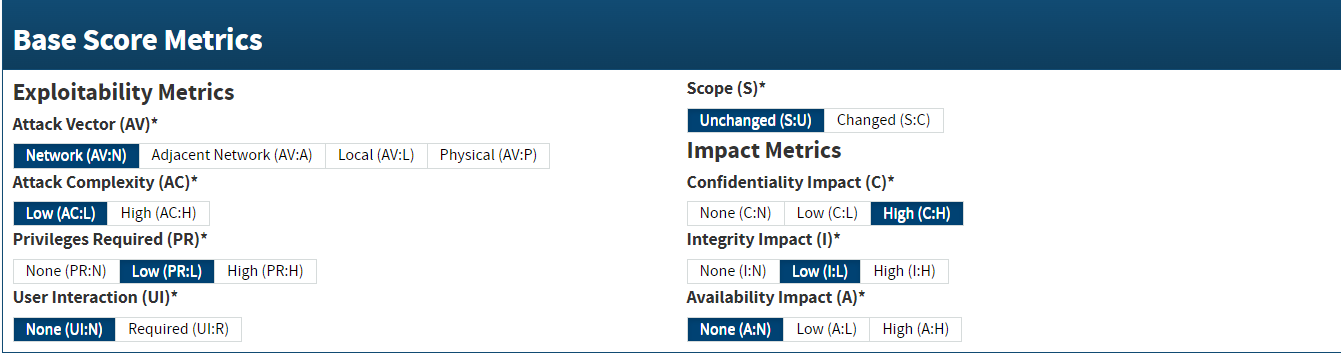
\includegraphics[keepaspectratio]{images/image28.png}}}

\subsection{\texorpdfstring{{Requisiti
dell\textquotesingle attaccante}}{Requisiti dell\textquotesingle attaccante}}\label{h.tovbgnlwqwie}

{L'attaccante deve avere un account con cui accedere al proprio carrello
e saper utilizzare il dev tool.}

\subsection{\texorpdfstring{{Gravità e
Impatti}}{Gravità e Impatti}}\label{h.r8oe422msqps}

{L'attaccante non può fare molti danni perché riesce ad accedere solo a
quali prodotti l'utente ha nel carrello, portando ad avere un impatto
sulla confidenzialità con una gravità abbastanza bassa.}

\end{document}
